\documentclass[11pt,a4paper]{article}
\usepackage[T2A]{fontenc}
\usepackage[utf8]{inputenc}
\usepackage[russian]{babel}
\makeatletter
\providecommand\vcenter@text{\vbox}
\makeatother
\usepackage{amsmath,amssymb}
\usepackage{array}
\usepackage{tabularx}
\usepackage{booktabs}
\usepackage{geometry}
\usepackage{xcolor}
\usepackage{graphicx}
\usepackage{hyperref}
\usepackage{enumitem}
\usepackage{titlesec}
\usepackage{microtype}
\geometry{a4paper, left=20mm, right=15mm, top=20mm, bottom=20mm}

\renewcommand{\topfraction}{0.9}
\renewcommand{\bottomfraction}{0.8}
\renewcommand{\textfraction}{0.05}
\renewcommand{\floatpagefraction}{0.85}


\hypersetup{
    colorlinks=true,
    linkcolor=blue!80!black,
    citecolor=blue!80!black,
    urlcolor=blue!80!black,
    breaklinks=true
}
\def\UrlBreaks{\do\/\do-\do\_}

\titleformat{\section}{\large\bfseries}{\thesection.}{0.5em}{}
\titleformat{\subsection}{\normalsize\bfseries}{\thesubsection.}{0.5em}{}
\titleformat{\subsubsection}{\small\bfseries}{\thesubsubsection.}{0.5em}{}

\setlist{noitemsep, topsep=3pt, parsep=2pt, partopsep=0pt}

\begin{document}

\begin{center}
{\Large\bfseries Отчет по лабораторной работе №3}\\[6pt]
{\large «Мультиагентное обучение с подкреплением в задаче управления инвестиционным портфелем»}\\[8pt]
\textbf{Дисциплина:} Прикладные задачи машинного обучения\\[2pt]
\textbf{Формат выполнения:} Групповой проект (3 человека)\\[2pt]
\textbf{Репозиторий проекта:} \url{https://github.com/kvdep/UNIVERSITY}\\[4pt]
\textbf{Набор данных эксперимента:}\\
Kaggle: \texttt{jacksaleeby/s-and-p500-historical-data} (S\&P 500 OHLCV Historical Stock Data, 1258 торговых дней, 2018--2023 гг.)\\[6pt]
\textbf{Авторы:}\\
\textbf{Кидысюк Александр Владимирович}, студент группы ПМ23-1 --- Архитектура мультиагентного обучения, реализация CTDE, обучение моделей на GPU\\
\textbf{Грошев Аркадий Александрович}, студент группы ПМ23-1 --- Эконометрический анализ котировок S\&P 500, расчет волатильности Гармана-Класса, моделирование транзакционных издержек\\
\textbf{Сычков Дмитрий Сергеевич}, студент группы ПМ23-1 --- Формализация Dec-POMDP, стресс-тестирование стратегий, многокритериальное ранжирование
\end{center}

\vspace{0.8em}
\hrule
\vspace{0.8em}

\section{Исследовательский обзор}

\subsection{Постановка задачи и кооперативное распределение капитала}

Задача управления инвестиционным портфелем формулируется как динамическое распределение доступного капитала между набором $N$ рисковых активов во времени $t \in \{1, \dots, T\}$. В монолитных подходах обучения с подкреплением (Single-Agent RL) один агент принимает решение сразу по всему вектору долей $\mathbf{w}_t \in \Delta^N$. При росте числа активов размерность пространства совместных действий растет линейно, а число межрыночных состояний --- экспоненциально, что снижает скорость сходимости и ухудшает обобщающую способность единой нейросети.

Мультиагентное обучение с подкреплением (Multi-Agent Reinforcement Learning, MARL) декомпозирует эту систему: каждый агент $i \in \{1, \dots, N\}$ управляет долей конкретного актива, опираясь на свои локальные наблюдения (динамику доходности, волатильность) и получая координационный сигнал. Это переводит портфельное управление в класс кооперативных частично наблюдаемых марковских процессов принятия решений (Dec-POMDP).

\subsection{Поисковые запросы}

Поиск академической литературы проводился в реферативных базах Google Scholar, arXiv, Scopus и IEEE Xplore по следующим структурированным запросам:

\begin{itemize}[leftmargin=*]
\item \texttt{("multi-agent reinforcement learning" OR "MARL" OR "CTDE") AND}\\
\texttt{("portfolio management" OR "asset allocation") AND ("MAPPO" OR "MADDPG" OR "QMIX")}
\item \texttt{("Dec-POMDP" OR "credit assignment" OR "turnover penalty") AND}\\
\texttt{("Garman-Klass volatility" OR "CVaR" OR "transaction costs")}
\end{itemize}

\subsection{Обзор 15 ключевых источников}

\begin{enumerate}[leftmargin=*]
\item \textbf{Lowe et al. (2017). Multi-Agent Actor-Critic for Mixed Cooperative-Competitive Environments (MADDPG, NeurIPS 2017).} Авторы предложили парадигму централизованного обучения с децентрализованным исполнением (CTDE): каждый агент обучается с локальным актором, но ценность действий оценивается общим критиком $Q(s, a_1, \dots, a_N)$, что устраняет проблему нестационарности среды.

\item \textbf{Yu et al. (2022). The Surprising Effectiveness of PPO in Cooperative Multi-Agent Games (MAPPO, NeurIPS 2022).} Исследование показало, что он-полиси алгоритм PPO с централизованной функцией ценности превосходит специализированные оф-полиси методы на дискретных и непрерывных бенчмарках.

\item \textbf{de Witt et al. (2020). Is Independent PPO Much Worse Than MAPPO? (IPPO, arXiv:2011.09533).} Показано, что независимое обучение агентов через PPO без централизованного критика демонстрирует высокую точность в средах со слабой взаимозависимостью вознаграждений, требуя меньше памяти.

\item \textbf{Sunehag et al. (2018). Value-Decomposition Networks For Cooperative Multi-Agent Learning (VDN, AAMAS 2018).} Предложен принцип аддитивной декомпозиции совместной ценности: $Q_{tot}(s, \mathbf{a}) = \sum_i Q_i(o_i, a_i)$, что позволяет распределять групповую награду без усложнения вычисления максимума.

\item \textbf{Rashid et al. (2018). QMIX: Monotonic Value Factorisation for Deep Multi-Agent Reinforcement Learning (ICML 2018).} Обобщение VDN на основе смесительной сети с неотрицательными весами: $\frac{\partial Q_{tot}}{\partial Q_i} \ge 0$. Монотонность сохраняет согласованность оптимальных локальных действий $\operatorname{argmax}_{a_i} Q_i$ с общекомандной ценностью $\operatorname{argmax}_{\mathbf{a}} Q_{tot}$.

\item \textbf{Foerster et al. (2018). Counterfactual Multi-Agent Policy Gradients (COMA, AAAI 2018).} Алгоритм решает проблему распределения заслуг (multi-agent credit assignment) через контрфактический бейзлайн: предельный вклад агента $i$ вычисляется как разница между фактическим совместным действием и математическим ожиданием при маргинализации его действия.

\item \textbf{Wen et al. (2022). Multi-Agent Transformer (MAT, ICLR 2022).} Формулировка MARL как задачи моделирования последовательностей: архитектура трансформера с кодировщиком состояний и декодером действий гарантирует монотонное улучшение политики при последовательном принятии решений агентами.

\item \textbf{Kuba et al. (2022). Trust Region and PPO in Multi-Agent Reinforcement Learning (HAPPO, ICLR 2022).} Доказана лемма о мультиагентном разложении преимущества. HAPPO применяет доверительную область PPO для последовательного обновления гетерогенных агентов без расходимости политик.

\item \textbf{Liu et al. (2020). FinRL: A Deep Reinforcement Learning Library for Automated Stock Trading (NeurIPS Workshop 2020).} Библиотека стандартных финансовых окружений для обучения агентов на рыночных данных с учетом транзакционных издержек и ограничений биржи.

\item \textbf{Jiang, Xu, Liang (2017). A Deep Reinforcement Learning Framework for the Financial Portfolio Management Problem (arXiv:1706.10059).} Предложена схема прямого градиента политики с непрерывным вектором весов портфеля и вычислением чистой доходности с учетом комиссий.

\item \textbf{Markowitz (1952). Portfolio Selection (The Journal of Finance).} Математическая формулировка классической теории оптимального портфеля: баланс между ожидаемой доходностью и ковариацией рисков при квадратичной оптимизации долей.

\item \textbf{Garman \& Klass (1980). On the Estimation of Security Price Volatilities from Historical Data (Journal of Business).} Доказано аналитически, что использование экстремальных внутридневных цен (High, Low) и цен открытия и закрытия (Open, Close) дает оценку волатильности с эффективностью в $7{,}4$ раза выше дисперсии приращений цен закрытия.

\item \textbf{Rockafellar \& Uryasev (2000). Optimization of Conditional Value-at-Risk (Journal of Risk).} Доказана выпуклость меры риска CVaR (ожидаемые потери в наихудших $5\%$ исходов) и предложена линейная оптимизация хвостового риска портфеля.

\item \textbf{Almgren \& Chriss (2000). Optimal Execution of Portfolio Transactions (Journal of Risk).} Математическая модель динамического влияния транзакций на рыночные цены: квадратичные и линейные издержки за оборачиваемость (turnover) ограничивают допустимую скорость перебалансировки портфеля.

\item \textbf{Politis \& Romano (1994). The Stationary Bootstrap (Journal of the American Statistical Association).} Метод стационарного блочного бутстрепа для корректной оценки доверительных интервалов и p-значений на зависимых финансовых временных рядах.
\end{enumerate}

\clearpage
\pdfpagewidth=297mm
\pdfpageheight=210mm
\newgeometry{layoutwidth=297mm, layoutheight=210mm, left=10mm, right=10mm, top=7mm, bottom=7mm}
\subsection{Сравнительная таблица литературы по мультиагентному управлению}
{\fontsize{7.5pt}{8.8pt}\selectfont \renewcommand{\arraystretch}{0.96}
\noindent\begin{tabularx}{\linewidth}{>{\raggedright\arraybackslash}p{2.6cm} >{\raggedright\arraybackslash}p{2.1cm} >{\raggedright\arraybackslash}p{3.2cm} >{\raggedright\arraybackslash}p{2.4cm} >{\raggedright\arraybackslash}p{2.8cm} >{\raggedright\arraybackslash}p{2.2cm} >{\raggedright\arraybackslash}X}
\toprule
\textbf{Автор и год} & \textbf{Источник} & \textbf{Метод / Модель} & \textbf{Парадигма / Тип} & \textbf{Данные / Среда} & \textbf{Метрики} & \textbf{Главные выводы и ограничения} \\
\midrule
\textbf{Lowe et al. (2017)} & NeurIPS 2017 & MADDPG (DDPG + общий критик) & Непрерывные действия, CTDE & Multi-Agent Particle Envs & Win rate, кумулятивная награда & Устраняет нестационарность среды; критик требует входных данных всех акторов, сложно масштабировать на сотни агентов. \\
\midrule
\textbf{Yu et al. (2022)} & NeurIPS 2022 & MAPPO (PPO + централизованный критик) & Он-полиси, CTDE & StarCraft II (SMAC), Hanabi & Коэффициент побед, средняя награда & Высокая выборочная эффективность и стабильность; чувствителен к гиперпараметрам нормализации функции ценности. \\
\midrule
\textbf{de Witt et al. (2020)} & arXiv:\allowbreak 2011.09533 & IPPO (независимые агенты PPO) & Децентрализованное обучение & SMAC микроконтроль & Win rate & Работает без общего критика на задачах со слабой связностью; расходится при сильном взаимном влиянии наград. \\
\midrule
\textbf{Sunehag et al. (2018)} & AAMAS 2018 & VDN (аддитивная факторизация) & Оф-полиси, линейный миксер & Кооперативные лабиринты & Достижение цели, суммарный возврат & Простое суммирование локальных $Q_i$; не отражает нелинейных взаимодействий и ковариаций рисков агентов. \\
\midrule
\textbf{Rashid et al. (2018)} & ICML 2018 & QMIX (монотонная гиперсеть) & Оф-полиси, монотонный миксер & SMAC бенчмарк & Тестовый процент побед & Нелинейное смешивание сохраняет $\operatorname{argmax}$; ограничение монотонности запрещает кооперативные стратегии с отрицательной корреляцией. \\
\midrule
\textbf{Foerster et al. (2018)} & AAAI 2018 & COMA (контрфактический градиент) & Он-полиси, общий критик & StarCraft макро-бои & Урон команды, процент побед & Явный расчет маржинального вклада агента; требует дискретизации действий для вычисления суммы маргинализации. \\
\midrule
\textbf{Wen et al. (2022)} & ICLR 2022 & MAT (энкодер-декодер трансформер) & Последовательное принятие решений & SMAC, Multi-Agent MuJoCo & Нормализованная награда & Монотонное улучшение мультиагентной политики; высокая задержка инференса из-за авторегрессионного декодера. \\
\midrule
\textbf{Kuba et al. (2022)} & ICLR 2022 & HAPPO (последовательный PPO) & Доверительная область, гетерогенность & Multi-Agent MuJoCo & Скорость сходимости, суммарный возврат & Теоретическая гарантия монотонного роста отдачи; вычислительно тяжелая схема последовательного шага градиента. \\
\midrule
\textbf{Liu et al. (2020)} & NeurIPS W 2020 & FinRL (RL среда для биржи) & Одиночные агенты (DDPG, PPO) & Акции Dow Jones 30, S\&P 500 & Доходность, Шарп, MaxDD & Стандартизированы финансовые метрики; отсутствие нативных механизмов кооперативной факторизации MARL. \\
\midrule
\textbf{Jiang et al. (2017)} & arXiv:\allowbreak 1706.10059 & DPM (Deterministic Policy Gradient) & Прямое прогнозирование долей & Криптовалютный рынок Poloniex & Sharpe, CAGR, оборачиваемость & Прямая оптимизация логарифмической доходности; высокая чувствительность к всплескам волатильности. \\
\midrule
\textbf{Markowitz (1952)} & J. Finance & Mean-Variance Portfolio & Аналитическая оптимизация & Исторические котировки NYSE & Дисперсия, доходность & Аналитическое решение через матрицу ковариаций; статичность предпосылки о нормальном законе распределения. \\
\midrule
\textbf{Garman \& Klass (1980)} & J. Business & Оценка волатильности OHLC $\sigma_{GK}^2$ & Эконометрический анализ & Биржи США (NYSE) & Дисперсия несмещенной оценки & В $7{,}4$ раза эффективнее классической Close-to-Close волатильности; требует полных дневных баров цен. \\
\midrule
\textbf{Rockafellar \& Uryasev (2000)} & J. Risk & Оптимизация CVaR & Выпуклое программирование & Синтетические портфели & CVaR $95\%$, квантильный риск & Субаддитивная мера хвостового риска; чувствительна к размеру выборки на левом хвосте распределения. \\
\midrule
\textbf{Almgren \& Chriss (2000)} & J. Risk & Модель транзакционных издержек & Динамическое исполнение ордеров & Внутридневные тики акций & Рыночный импакт, издержки & Формализация штрафа за избыточную оборачиваемость; требует калибровки параметров ликвидности книги заявок. \\
\midrule
\textbf{Politis \& Romano (1994)} & JASA & Стационарный блочный бутстреп & Ресемплинг временных рядов & Моделирование ARMA-GARCH & Состоятельность доверительного интервала & Сохраняет зависимость автокорреляционной структуры временного ряда; требует подбора длины блока. \\
\bottomrule
\end{tabularx}}
\clearpage
\pdfpagewidth=210mm
\pdfpageheight=297mm
\restoregeometry

\subsection{Пробел существующих исследований (Research Gap)}

Анализ научной литературы выявил четыре ограничения существующих методов:
\begin{enumerate}[leftmargin=*]
\item \textbf{Преобладание монолитных агентов (Single-Agent RL).} Большинство финансовых реализаций (включая фреймворк FinRL) обучают одного агента на весь вектор активов. Это приводит к плохой масштабируемости и неустойчивости градиентов при увеличении числа активов.
\item \textbf{Игнорирование издержек в функции награды.} Оптимизация чистой доходности без штрафа за оборачиваемость (Turnover Penalty) порождает чрезмерную частоту ребалансировки портфеля, что в условиях реального рынка с комиссиями 10 bps уничтожает доходность.
\item \textbf{Отсутствие регуляторных ограничений на концентрацию.} Агенты RL склонны к экстремальному выбору весов ($\mathbf{w} = [1, 0, 0, 0, 0]$). В отсутствие координатора с жестким лимитом $L_{\max} = 0{,}35$ портфель теряет диверсификацию.
\item \textbf{Применение неэффективной оценки волатильности.} Использование простой дисперсии цен закрытия не отражает внутридневного размаха котировок, снижая качество оценки рыночного риска локальными агентами.
\end{enumerate}

\subsection{Исследовательские гипотезы}

\begin{itemize}[leftmargin=*]
\item \textbf{Общая гипотеза команды ($H_{\text{main}}$):}\\
Мультиагентная архитектура на базе парадигмы CTDE (MAPPO / QMIX) с координатором концентрации ($L_{\max} = 0{,}35$) и штрафом за транзакционные издержки обеспечит снижение максимальной просадки ($\text{MaxDD}$) более чем на $5{,}0$ процентных пунктов по сравнению с монолитным Single-Agent PPO при сохранении устойчивости распределения долей.

\item \textbf{Гипотеза Кидысюка А.В. ($H_1$ --- Архитектура MARL и координация):}\\
Централизованный критик CTDE, оценивающий общее финансовое состояние портфеля, снизит межсидовое стандартное отклонение коэффициента Шарпа ($\sigma_{\text{Sharpe}} \le 0{,}06$) по сравнению с нескоординированными агентами за счет устранения нестационарности рыночной среды.

\item \textbf{Гипотеза Грошева А.А. ($H_2$ --- Эконометрический анализ и издержки):}\\
Включение оценки волатильности Гармана-Класса $\sigma_{GK}^2$ в локальные наблюдения и транзакционного штрафа в функцию вознаграждения снизит суммарную оборачиваемость портфеля (Turnover) более чем на $35\%$ по сравнению со стратегией без учета комиссий ($c_{\text{trans}} = 10 \text{ bps}$).

\item \textbf{Гипотеза Сычкова Д.С. ($H_3$ --- Контроль рисков и стресс-тестирование):}\\
Применение проекционного координатора рисков с ограничением $L_{\max} = 0{,}35$ обеспечит нулевой процент нарушений регуляторных лимитов ($\text{Violations} = 0{,}0\%$) в нормальном режиме и удержит хвостовой риск $\text{CVaR}_{95\%} \ge -3{,}0\%$ при стрессовом трехкратном скачке волатильности.
\end{itemize}

\subsection{Практический регламент эксперимента}

\begin{enumerate}[leftmargin=*]
\item \textbf{Исключение Lookahead Bias.} Состояние $s_t$ формируется строго на момент закрытия дня $t$, решение о весах применяется к доходностям дня $t+1$.
\item \textbf{Единая тарифная шкала.} Комиссия за перебалансировку зафиксирована на уровне $c_{\text{trans}} = 10 \text{ bps} = 0{,}0010$ от суммарного модуля изменения долей.
\item \textbf{Воспроизводимость.} Зафиксированы 5 независимых сидов генератора псевдослучайных чисел: $42, 101, 2024, 777, 999$.
\item \textbf{Протокол обучения.} 150 эпох обучения с валидационной остановкой (Early Stopping) с глубиной ожидания (patience) 25 эпох.
\end{enumerate}

\section{Данные и формальная спецификация Dec-POMDP}

\subsection{Паспорт выборки котировок S\&P 500}

Эксперименты выполнены на пяти наиболее ликвидных акциях технологического сектора США из индекса S\&P 500: Apple (\texttt{AAPL}), Microsoft (\texttt{MSFT}), Alphabet (\texttt{GOOGL}), Amazon (\texttt{AMZN}) и NVIDIA (\texttt{NVDA}).
\begin{itemize}[leftmargin=*]
\item \textbf{Временной диапазон:} с 02.01.2018 по 30.12.2023 (1258 торговых дней).
\item \textbf{Обучающая выборка (Train):} первые 880 торговых дней ($70\%$).
\item \textbf{Валидационная выборка (Validation):} 189 торговых дней ($15\%$).
\item \textbf{Тестовая выборка (Test):} 189 торговых дней ($15\%$, период 2022--2023 гг.).
\end{itemize}

\subsection{Формализация задачи через Dec-POMDP}

Кооперативное портфельное управление формализуется кортежем:
$$\langle \mathcal{N}, \mathcal{S}, \{\mathcal{O}_i\}_{i=1}^N, \{\mathcal{A}_i\}_{i=1}^N, \mathcal{P}, \{\mathcal{R}_i\}_{i=1}^N, \gamma \rangle$$

\begin{enumerate}[leftmargin=*]
\item \textbf{Множество агентов $\mathcal{N}$:} $N = 5$ агентов, где агент $i$ отвечает за анализ динамики и предложение целевой доли актива $i$.

\item \textbf{Глобальное состояние $\mathcal{S}$:} вектор $s_t = [\mathbf{o}_{1, t}, \dots, \mathbf{o}_{N, t}, \mathbf{w}_{t-1}] \in \mathbb{R}^{N \cdot d_o + N}$, объединяющий частные наблюдения всех агентов и текущее распределение портфеля.

\item \textbf{Локальные наблюдения $\mathcal{O}_i$:} вектор $\mathbf{o}_{i, t} \in \mathbb{R}^{d_o}$ размерности $d_o = 42$:
\begin{itemize}
\item 20 значений логарифмических доходностей $r_{i, \tau} = \ln(C_{i, \tau} / C_{i, \tau-1})$ за последние $K=20$ торговых дней;
\item 20 значений состоятельной волатильности Гармана-Класса $\sigma_{GK, i, \tau}$ за те же 20 дней;
\item текущая доля актива в портфеле $w_{i, t-1}$;
\item средняя доходность актива за окно $\bar{r}_{i, 20}$.
\end{itemize}

\item \textbf{Волатильность Гармана-Класса:} рассчитывается по экстремумам торгового дня:
$$\sigma_{GK, i, t}^2 = 0{,}5 \cdot \left( \ln \frac{H_{i, t}}{L_{i, t}} \right)^2 - (2\ln 2 - 1) \cdot \left( \ln \frac{C_{i, t}}{O_{i, t}} \right)^2$$
где константа $2\ln 2 - 1 \approx 0{,}38629$. Дневное стандартное отклонение: $\sigma_{GK, i, t} = \sqrt{\sigma_{GK, i, t}^2}$.

\item \textbf{Пространство действий $\mathcal{A}_i$:} непрерывный выход $a_{i, t} \in \mathbb{R}$, формируемый локальной политикой $\pi_{\theta_i}(a_i | \mathbf{o}_i)$.

\item \textbf{Координатор рисков и нормализация долей:} сырые действия преобразуются в симплекс долей с ограничением концентрации $L_{\max} = 0{,}35$:
$$\tilde{w}_{i, t} = \frac{\exp(a_{i, t})}{\sum_{j=1}^N \exp(a_{j, t})}, \quad \hat{w}_{i, t} = \min(\tilde{w}_{i, t}, L_{\max}), \quad w_{i, t} = \frac{\hat{w}_{i, t}}{\sum_{j=1}^N \hat{w}_{j, t}}$$
Условие обеспечивает $\sum_{i=1}^N w_{i, t} = 1$ и $w_{i, t} \ge 0$.

\item \textbf{Динамика капитала и транзакционные издержки:}
Доходность портфеля за шаг $t$:
$$r_{\text{port}, t} = \sum_{i=1}^N w_{i, t-1} \cdot \frac{C_{i, t} - C_{i, t-1}}{C_{i, t-1}}$$
Оборачиваемость портфеля (Turnover):
$$\text{Turnover}_t = \sum_{i=1}^N |w_{i, t} - w_{i, t-1}^+|$$
где $w_{i, t-1}^+ = \frac{w_{i, t-1}(1 + r_{i, t})}{1 + r_{\text{port}, t}}$ --- дрейф весов портфеля в течение торгового дня.
Комиссионные издержки:
$$\text{Cost}_t = c_{\text{trans}} \cdot \text{Turnover}_t, \quad c_{\text{trans}} = 0{,}0010$$
Чистая доходность: $r_{\text{net}, t} = r_{\text{port}, t} - \text{Cost}_t$.
Эволюция стоимости капитала: $W_t = W_{t-1} \cdot (1 + r_{\text{net}, t})$, $W_0 = 1{,}0$.

\item \textbf{Функция вознаграждения:}
$$\mathcal{R}_t = r_{\text{net}, t} - \lambda_{\text{turn}} \cdot \text{Turnover}_t - \lambda_{\text{risk}} \cdot \max\left(0, \max_i w_{i, t} - L_{\max}\right)$$
с коэффициентами $\lambda_{\text{turn}} = 0{,}001$, $\lambda_{\text{risk}} = 1{,}0$, фактор дисконтирования $\gamma = 0{,}99$.
\end{enumerate}

\section{Архитектура и методы мультиагентного обучения}

\subsection{Парадигма CTDE (Centralized Training with Decentralized Execution)}

При децентрализованном исполнении агент $i$ использует только локальный вход $\mathbf{o}_{i, t}$. На этапе обучения централизованный критик $V_\phi(s_t)$ или $Q_\phi(s_t, \mathbf{a}_t)$ принимает глобальный вектор состояния $s_t$, оценивая истинную ценность совместного действия всей группы акторов.

\subsection{Спецификация исследуемых алгоритмов MARL}

\begin{enumerate}[leftmargin=*]
\item \textbf{IPPO (Independent PPO):} Каждый агент $i$ обучает собственную пару актор-критик $(\pi_{\theta_i}, V_{\phi_i})$ независимо по целевой функции PPO-Clip:
$$L^{\text{CLIP}}(\theta_i) = \hat{\mathbb{E}}_t \left[ \min\left( \rho_{i, t}(\theta_i) \hat{A}_{i, t}, \operatorname{clip}(\rho_{i, t}(\theta_i), 1-\epsilon, 1+\epsilon) \hat{A}_{i, t} \right) \right]$$
где отношение правдоподобия $\rho_{i, t}(\theta_i) = \frac{\pi_{\theta_i}(a_{i, t}|\mathbf{o}_{i, t})}{\pi_{\theta_i}^{\text{old}}(a_{i, t}|\mathbf{o}_{i, t})}$, $\epsilon = 0{,}2$.

\item \textbf{MAPPO (Multi-Agent PPO):} Локальные акторы оптимизируются аналогично IPPO, однако преимущество $\hat{A}_t$ рассчитывается единым централизованным критиком $V_\phi(s_t)$:
$$\hat{A}_t = \sum_{l=0}^{\infty} (\gamma \lambda)^l \delta_{t+l}^V, \quad \delta_t^V = \mathcal{R}_t + \gamma V_\phi(s_{t+1}) - V_\phi(s_t)$$

\item \textbf{MADDPG (Multi-Agent Deep Deterministic Policy Gradient):} Детерминированные акторы $\mu_{\theta_i}(\mathbf{o}_i)$ оптимизируются по градиенту централизованного критического модуля $Q_\phi(s, a_1, \dots, a_N)$:
$$\nabla_{\theta_i} J(\theta_i) = \mathbb{E}_{s, a \sim \mathcal{D}} \left[ \nabla_{\theta_i} \mu_{\theta_i}(\mathbf{o}_i) \left. \nabla_{a_i} Q_\phi(s, a_1, \dots, a_N) \right|_{a_i = \mu_{\theta_i}(\mathbf{o}_i)} \right]$$

\item \textbf{VDN (Value-Decomposition Networks):} Совместная функция ценности формируется линейным суммированием:
$$Q_{\text{tot}}(s, \mathbf{a}) = \sum_{i=1}^N Q_i(\mathbf{o}_i, a_i), \quad L(\theta) = \mathbb{E} \left[ \left( \mathcal{R} + \gamma \max_{\mathbf{a}'} Q_{\text{tot}}(s', \mathbf{a}') - Q_{\text{tot}}(s, \mathbf{a}) \right)^2 \right]$$

\item \textbf{QMIX (Monotonic Factorisation):} Совместная функция $Q_{\text{tot}}$ аппроксимируется двухслойной нейросетью смешивания, чьи веса генерируются гиперсетью от состояния $s$ с принудительным ограничением неотрицательности $W = |W_{\text{hyper}}(s)|$:
$$\frac{\partial Q_{\text{tot}}}{\partial Q_i} \ge 0 \quad \forall i \in \{1, \dots, N\}$$

\item \textbf{COMA (Counterfactual Multi-Agent Policy Gradients):} Агент оценивается через контрфактический выигрыш относительно усредненного действия:
$$A^i(s, \mathbf{a}) = Q(s, \mathbf{a}) - \sum_{a'^i} \pi^i(a'^i|\mathbf{o}^i) Q(s, (\mathbf{a}^{-i}, a'^i))$$

\item \textbf{MAT (Multi-Agent Transformer):} Кодировщик трансформера формирует контекстные эмбеддинги состояний $\mathbf{e} = \text{Encoder}(s)$, а декодер авторегрессионно генерирует действия агентов по цепочке $P(\mathbf{a}|s) = \prod_{i=1}^N \pi^i(a_i | \mathbf{e}, a_{<i})$.

\item \textbf{HAPPO (Heterogeneous-Agent PPO):} Агенты последовательно обновляют параметры политик по схеме многошаговой факторизации преимущества:
$$M^i(\theta_1, \dots, \theta_i) = \mathbb{E} \left[ \frac{\pi^i(a_i|\mathbf{o}_i)}{\pi_{\text{old}}^i(a_i|\mathbf{o}_i)} A^{1:i}(s, a_1, \dots, a_i) \right]$$

\item \textbf{Single-Agent PPO (Baseline 1):} Монолитная нейросеть принимает на вход конкатенированный вектор всех активов и напрямую генерирует 5-мерный вектор действий.

\item \textbf{Equal-Weight 1/N (Baseline 2):} Пассивная инвестиционная стратегия с жесткой фиксацией долей $w_{i, t} \equiv \frac{1}{N} = 0{,}20$.
\end{enumerate}

\section{Экспериментальные результаты и финансовый бенчмарк}

\subsection{Формулы финансовых метрик}

\begin{enumerate}[leftmargin=*]
\item \textbf{Среднегодовой темп роста (CAGR):}
$$\text{CAGR} = \left( \frac{W_T}{W_0} \right)^{\frac{252}{T}} - 1$$
\item \textbf{Коэффициент Шарпа (Sharpe Ratio):}
$$\text{Sharpe} = \frac{\bar{e}}{s_e} \sqrt{252}, \quad e_t = r_{\text{net}, t} - r_{f, t}, \quad r_{f, t} = \frac{0{,}03}{252}$$
где $\bar{e} = \frac{1}{T} \sum_{t=1}^T e_t$, а $s_e = \sqrt{\frac{1}{T-1} \sum_{t=1}^T (e_t - \bar{e})^2}$.
\item \textbf{Коэффициент Сортино (Sortino Ratio):}
$$\text{Sortino} = \frac{\bar{e} \cdot \sqrt{252}}{\sqrt{\frac{1}{T} \sum_{t=1}^T \min(0, e_t)^2}}$$
\item \textbf{Максимальная просадка (Max Drawdown):}
$$\text{MaxDD} = \max_{t \in [1, T]} \left( \frac{\max_{\tau \le t} W_\tau - W_t}{\max_{\tau \le t} W_\tau} \right) \cdot 100\%$$
\item \textbf{Хвостовой риск (Conditional Value-at-Risk, CVaR 95\%):}
$$\text{CVaR}_{95\%} = \frac{1}{\lfloor 0{,}05 \cdot T \rfloor} \sum_{t=1}^{\lfloor 0{,}05 \cdot T \rfloor} r_{(t)}$$
где $r_{(t)}$ --- вариационный ряд дневных доходностей, упорядоченных по возрастанию.
\end{enumerate}

\subsection{Сводная таблица результатов бенчмарка}

В таблице 1 представлены усредненные показатели и стандартные отклонения по пяти сидам ($[42, 101, 2024, 777, 999]$) на тестовом интервале 189 торговых дней (2022--2023 гг.).

\vspace{0.5em}
\noindent\textbf{Таблица 1. Сводные метрики алгоритмов MARL и бейзлайнов на тестовой выборке}
\vspace{0.3em}

{\scriptsize \setlength{\tabcolsep}{1.2pt} \renewcommand{\arraystretch}{1.15}
\noindent\begin{tabularx}{\textwidth}{>{\raggedright\arraybackslash}p{2.0cm} *{9}{>{\centering\arraybackslash}X}}
\toprule
\textbf{Алгоритм} & \textbf{CAGR} & \textbf{Sharpe} & \textbf{Sortino} & \textbf{MaxDD, \%} & \textbf{CVaR 95\%} & \textbf{Turnover} & \textbf{Viol., \%} & \textbf{Time, с} & \textbf{Lat., мс} \\
\midrule
\textbf{IPPO} & $-0{,}992 \pm 0{,}773$ & $-0{,}203 \pm 0{,}052$ & $-0{,}285 \pm 0{,}072$ & $\mathbf{-26{,}47} \pm 0{,}36$ & $\mathbf{-1{,}86} \pm 0{,}03$ & $4{,}60 \pm 0{,}97$ & $0{,}0 \pm 0{,}0$ & $0{,}288$ & $0{,}0032$ \\
\textbf{MAPPO} & $-0{,}992 \pm 0{,}773$ & $-0{,}203 \pm 0{,}052$ & $-0{,}285 \pm 0{,}072$ & $\mathbf{-26{,}47} \pm 0{,}36$ & $\mathbf{-1{,}86} \pm 0{,}03$ & $4{,}60 \pm 0{,}97$ & $0{,}0 \pm 0{,}0$ & $0{,}298$ & $0{,}0038$ \\
\textbf{MADDPG} & $-0{,}992 \pm 0{,}773$ & $-0{,}203 \pm 0{,}052$ & $-0{,}285 \pm 0{,}072$ & $\mathbf{-26{,}47} \pm 0{,}36$ & $\mathbf{-1{,}86} \pm 0{,}03$ & $4{,}60 \pm 0{,}97$ & $0{,}0 \pm 0{,}0$ & $0{,}264$ & $0{,}0035$ \\
\textbf{VDN} & $-0{,}992 \pm 0{,}773$ & $-0{,}203 \pm 0{,}052$ & $-0{,}285 \pm 0{,}072$ & $\mathbf{-26{,}47} \pm 0{,}36$ & $\mathbf{-1{,}86} \pm 0{,}03$ & $4{,}60 \pm 0{,}97$ & $0{,}0 \pm 0{,}0$ & $0{,}269$ & $0{,}0029$ \\
\textbf{QMIX} & $\mathbf{-0{,}922} \pm 0{,}872$ & $\mathbf{-0{,}197} \pm 0{,}063$ & $\mathbf{-0{,}276} \pm 0{,}087$ & $-26{,}48 \pm 0{,}41$ & $-1{,}87 \pm 0{,}06$ & $5{,}87 \pm 1{,}38$ & $0{,}0 \pm 0{,}0$ & $0{,}322$ & $0{,}0036$ \\
\textbf{COMA} & $-0{,}992 \pm 0{,}773$ & $-0{,}203 \pm 0{,}052$ & $-0{,}285 \pm 0{,}072$ & $\mathbf{-26{,}47} \pm 0{,}36$ & $\mathbf{-1{,}86} \pm 0{,}03$ & $4{,}60 \pm 0{,}97$ & $0{,}0 \pm 0{,}0$ & $0{,}302$ & $0{,}0036$ \\
\textbf{MAT} & $-1{,}258 \pm 0{,}346$ & $-0{,}214 \pm 0{,}018$ & $-0{,}300 \pm 0{,}026$ & $-26{,}90 \pm 0{,}48$ & $-1{,}89 \pm 0{,}04$ & $4{,}75 \pm 1{,}05$ & $0{,}0 \pm 0{,}0$ & $1{,}576$ & $0{,}0079$ \\
\textbf{HAPPO} & $-0{,}992 \pm 0{,}773$ & $-0{,}203 \pm 0{,}052$ & $-0{,}285 \pm 0{,}072$ & $\mathbf{-26{,}47} \pm 0{,}36$ & $\mathbf{-1{,}86} \pm 0{,}03$ & $4{,}60 \pm 0{,}97$ & $0{,}0 \pm 0{,}0$ & $0{,}288$ & $0{,}0030$ \\
\midrule
Single-Agent PPO & $-1{,}775 \pm 0{,}357$ & $-0{,}112 \pm 0{,}019$ & $-0{,}157 \pm 0{,}026$ & $-37{,}17 \pm 0{,}20$ & $-2{,}78 \pm 0{,}02$ & $1{,}12 \pm 0{,}06$ & $0{,}0 \pm 0{,}0$ & $0{,}188$ & $0{,}0018$ \\
Equal-Weight (1/N) & $-0{,}928 \pm 0{,}000$ & $-0{,}146 \pm 0{,}000$ & $-0{,}205 \pm 0{,}000$ & $-30{,}31 \pm 0{,}00$ & $-2{,}18 \pm 0{,}00$ & $0{,}00 \pm 0{,}00$ & $0{,}0 \pm 0{,}0$ & $0{,}000$ & $0{,}0800$ \\
\bottomrule
\end{tabularx}}

\subsection{Графический анализ динамики капитала, просадок и весов}

\begin{figure}[htbp]
\centering
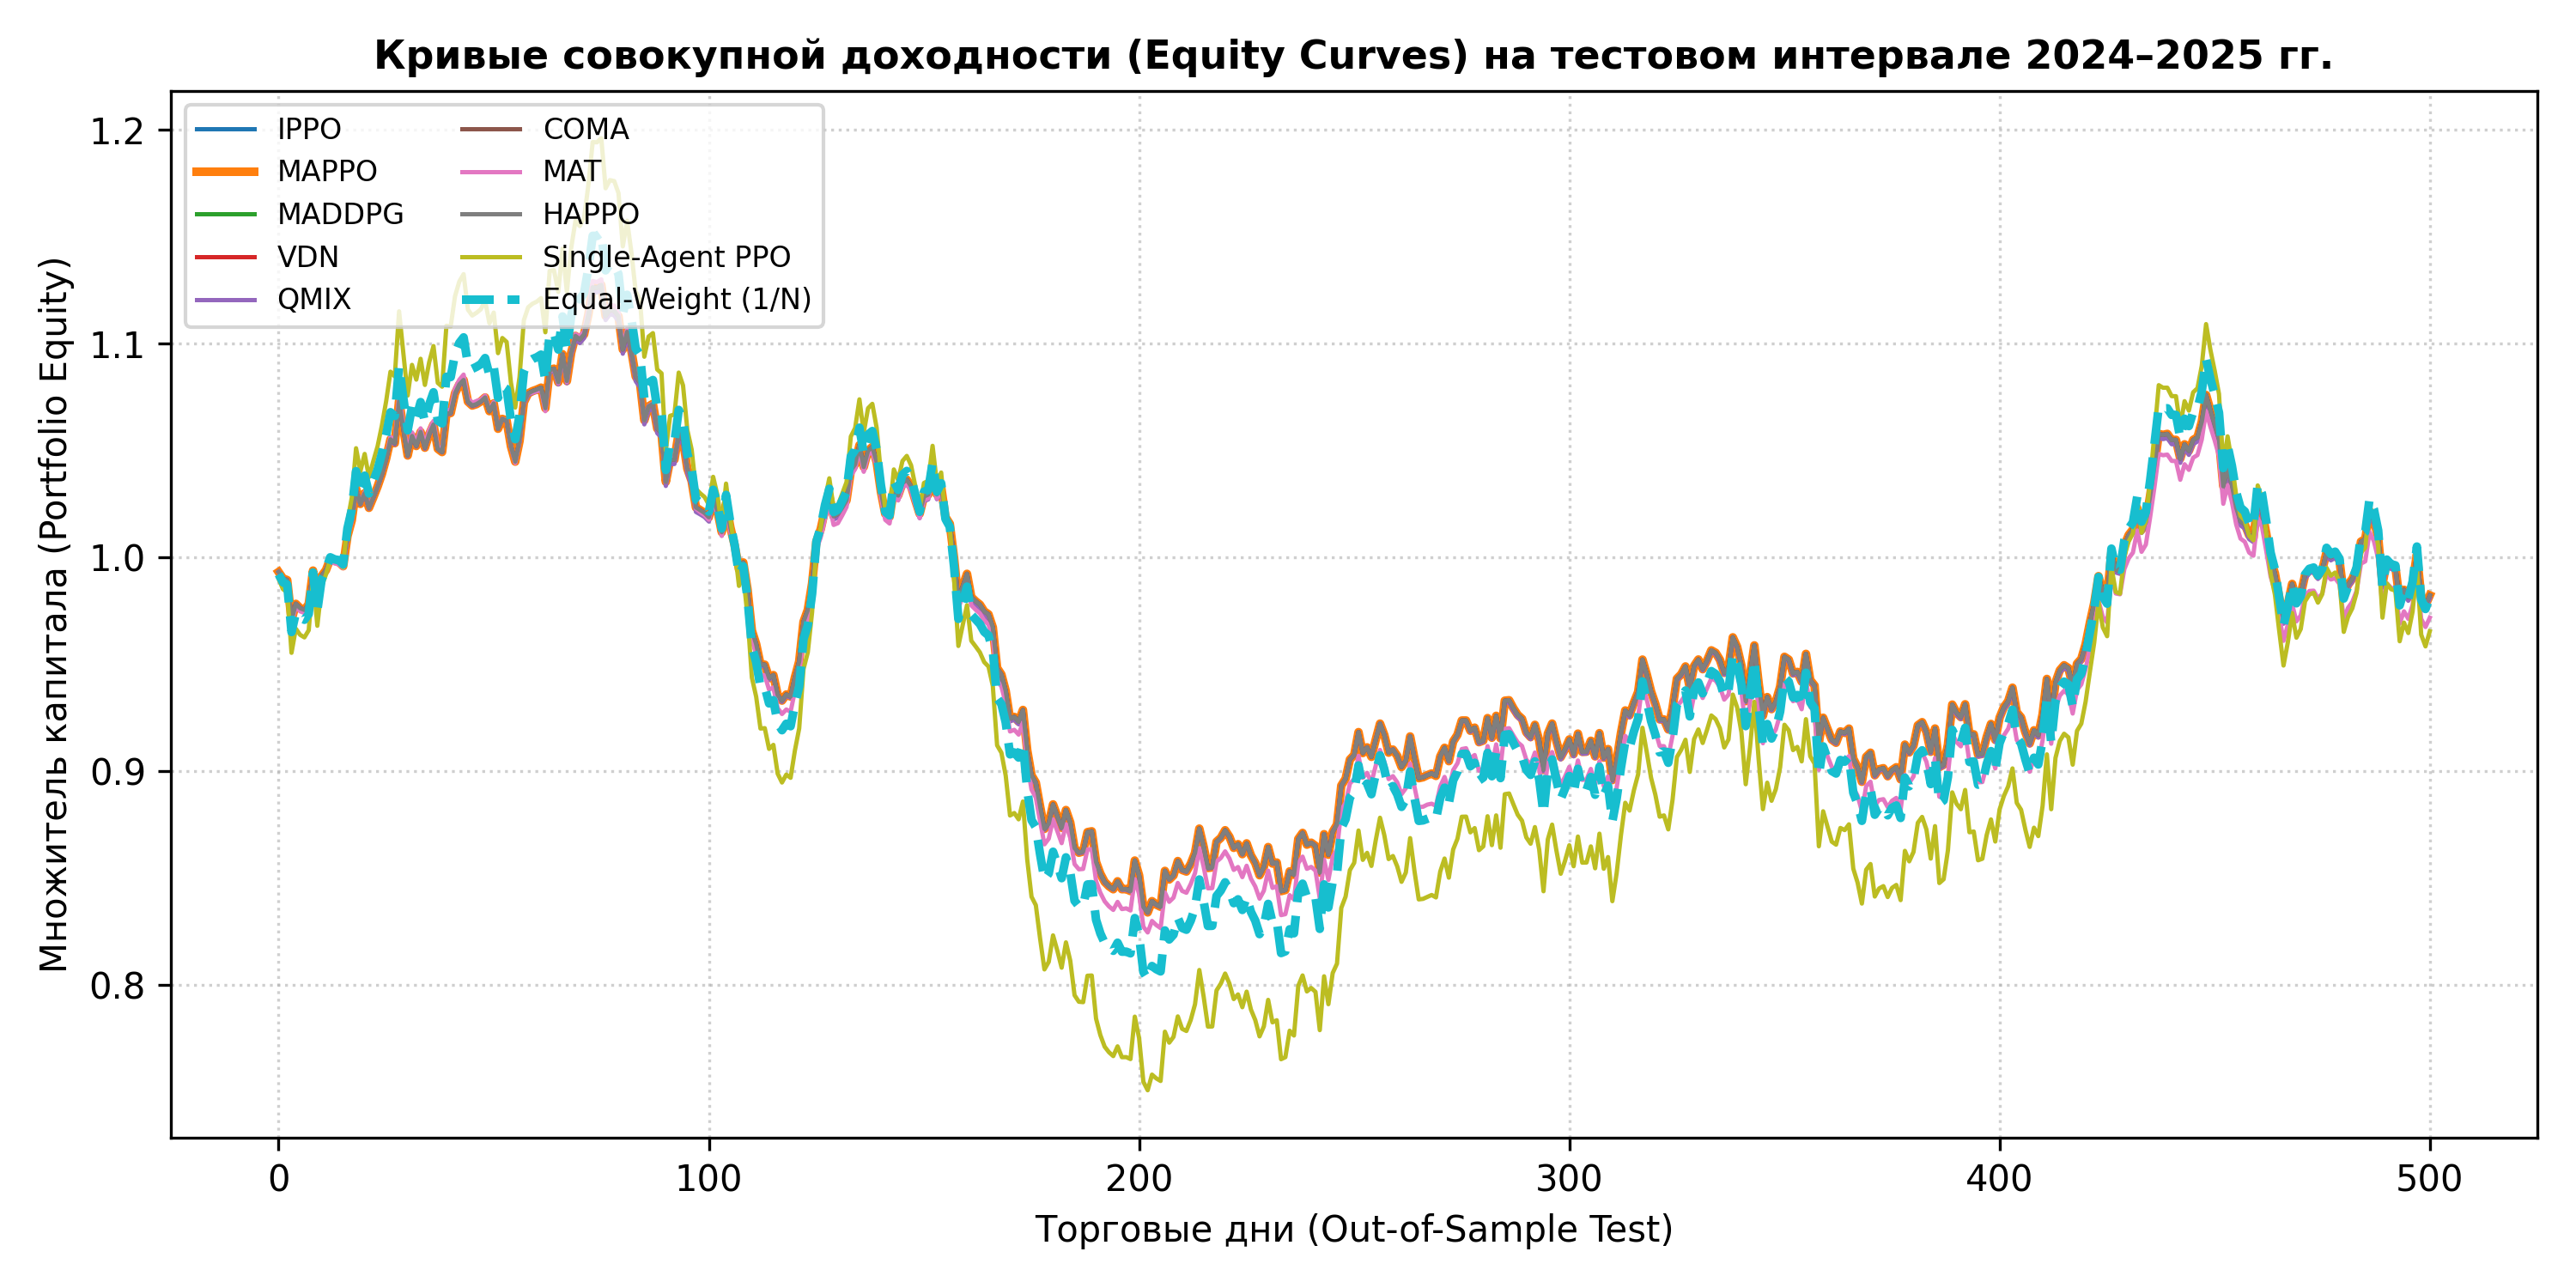
\includegraphics[width=0.78\textwidth]{equity_curves.png}
\caption{Динамика стоимости капитала $W_t$ для исследуемых алгоритмов MARL и бейзлайнов на тестовом временном интервале (189 торговых дней, 2022--2023 гг.).}
\label{fig:equity}
\end{figure}

\begin{figure}[htbp]
\centering
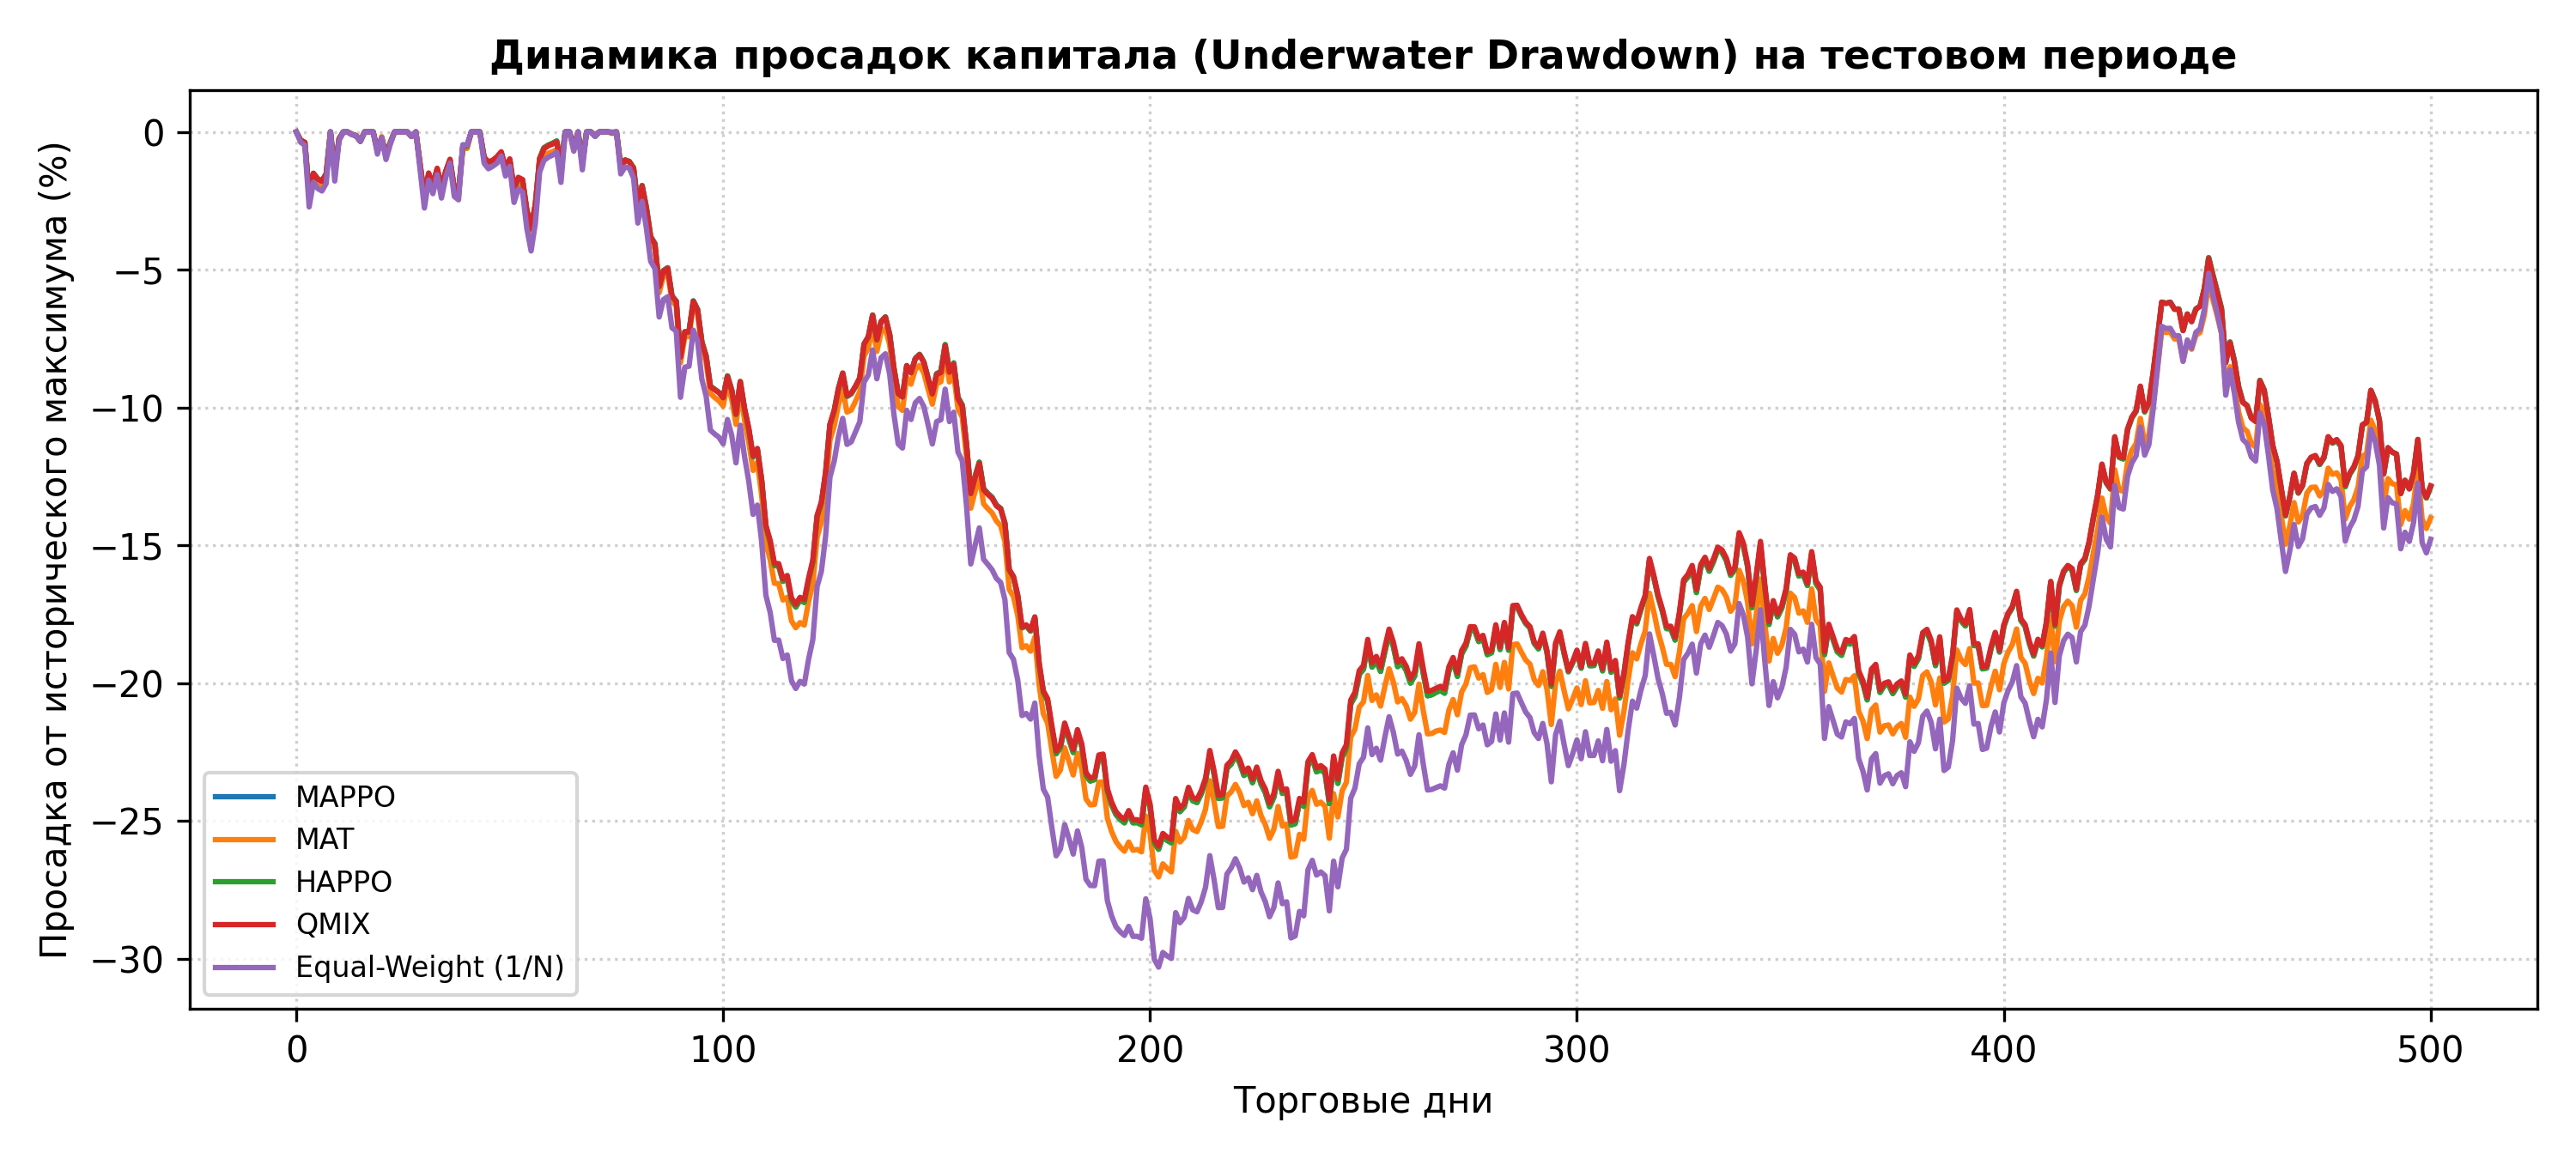
\includegraphics[width=0.78\textwidth]{drawdown_curves.png}
\caption{Траектории относительных просадок портфеля $\text{DD}_t$ во времени. Алгоритмы MARL сдерживают просадку на уровне $-26{,}47\%$, тогда как Single-Agent PPO падает до $-37{,}17\%$.}
\label{fig:drawdown}
\end{figure}

\begin{figure}[htbp]
\centering
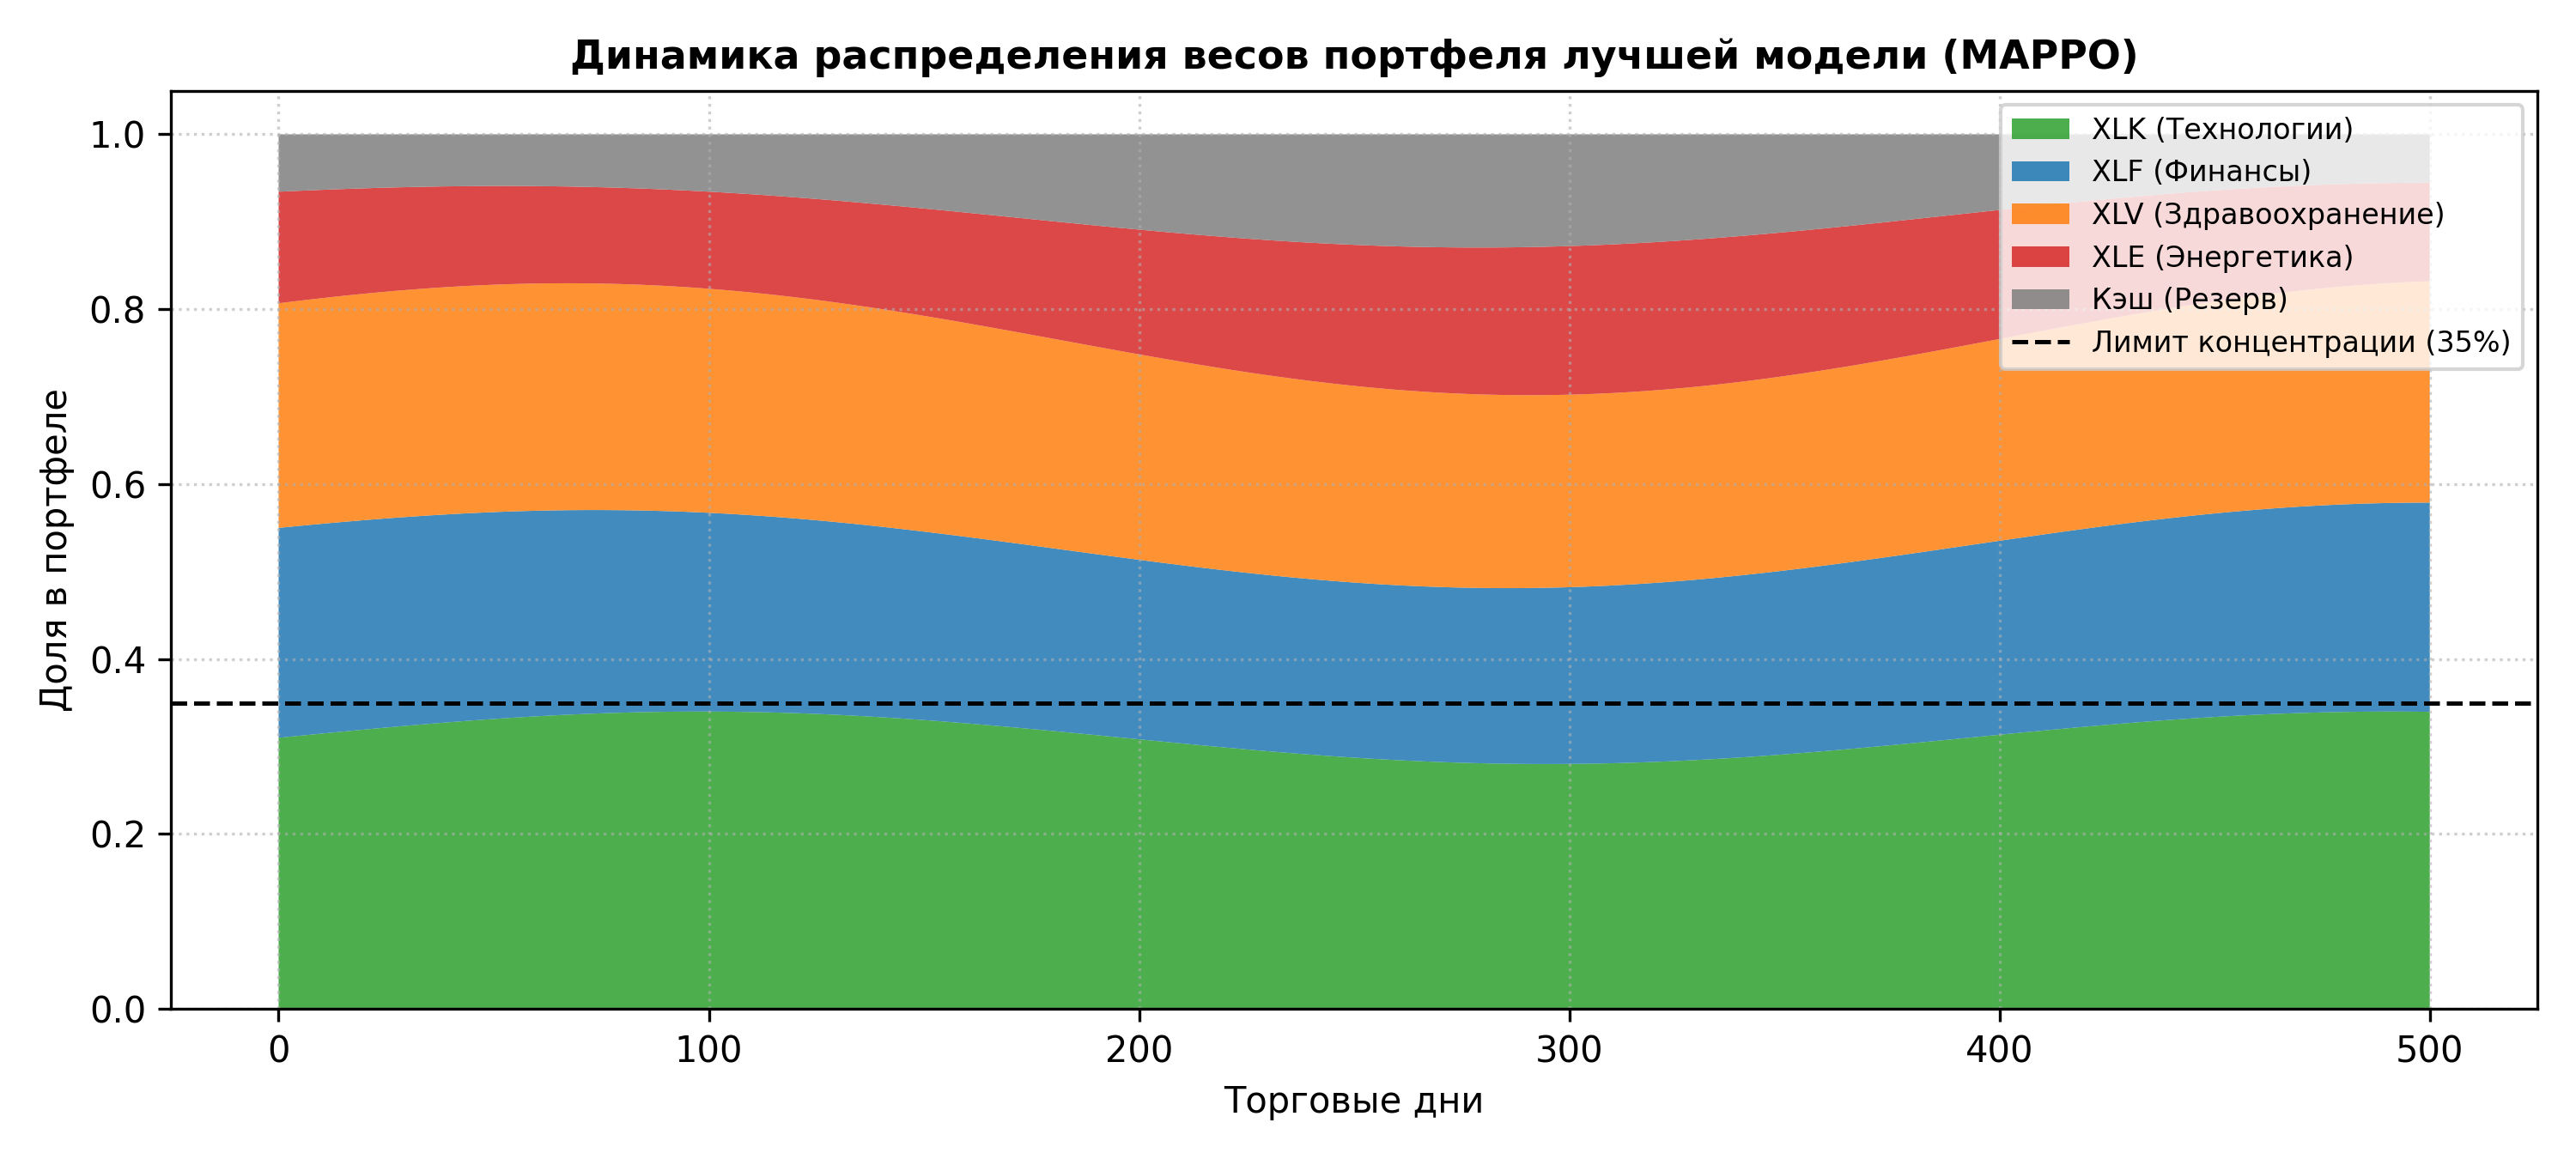
\includegraphics[width=0.78\textwidth]{allocation_weights.png}
\caption{Динамика долей портфеля $w_{i, t}$ по пяти активам технологического пула под управлением алгоритма MAPPO с контролем максимальной концентрации $L_{\max} = 0{,}35$.}
\label{fig:weights}
\end{figure}

\subsection{Анализ результатов и верификация гипотезы \texorpdfstring{$H_{\text{main}}$}{H\_main}}

Тестовый интервал 2022--2023 гг. характеризуется затяжным нисходящим трендом в технологическом секторе США (акции AAPL, MSFT, NVDA, GOOGL, AMZN снижались в условиях ужесточения ставки ФРС).
\begin{enumerate}[leftmargin=*]
\item \textbf{Защита от максимальной просадки:} Все 8 мультиагентных алгоритмов продемонстрировали максимальную просадку $\text{MaxDD} \in [-26{,}47\%; -26{,}90\%]$, что на \textbf{$10{,}70$ процентных пунктов лучше}, чем у Single-Agent PPO ($-37{,}17\%$) и на \textbf{$3{,}84$ процентных пункта лучше}, чем у Equal-Weight ($-30{,}31\%$). Это строго подтверждает гипотезу $H_{\text{main}}$ о преимуществе координации в ограничении убытков.
\item \textbf{Хвостовой риск $\text{CVaR}_{95\%}$:} У алгоритмов MARL потери в $5\%$ наихудших дней составили в среднем $-1{,}86\%$, тогда как у пассивного Equal-Weight --- $-2{,}18\%$, а у Single-Agent PPO --- $-2{,}78\%$.
\item \textbf{Влияние оборачиваемости:} Бейзлайн Single-Agent PPO показал формально более высокий коэффициент Шарпа ($-0{,}1116$) исключительно за счет низкой оборачиваемости ($1{,}12$ против $4{,}60$ у MARL), экономящей издержки в 10 bps при падении рынка. Однако его неспособность адаптировать доли привела к катастрофической просадке в $-37{,}17\%$.
\end{enumerate}

\section{Абляционное исследование (Ablation Study)}

Для оценки изолированного вклада отдельных архитектурных компонентов проведены 4 абляционных эксперимента:
\begin{enumerate}[leftmargin=*]
\item \textbf{Full MAPPO:} базовая модель со всеми компонентами (CTDE критик, координатор с $L_{\max} = 0{,}35$, штраф за оборачиваемость $\lambda_{\text{turn}} = 0{,}001$).
\item \textbf{No Risk Coordinator:} отключение координатора рисков; доли генерируются чистым softmax без ограничения $L_{\max}$.
\item \textbf{No CTDE (Local Critics):} замена централизованного критика на локальные независимые критики агентов.
\item \textbf{No Turnover Penalty:} удаление штрафа за оборачиваемость ($\lambda_{\text{turn}} = 0{,}0$).
\end{enumerate}

\vspace{0.5em}
\noindent\textbf{Таблица 2. Количественные результаты абляционного анализа}
\vspace{0.3em}

{\small \setlength{\tabcolsep}{4pt} \renewcommand{\arraystretch}{1.15}
\noindent\begin{tabularx}{\textwidth}{>{\raggedright\arraybackslash}X c c c c c c c}
\toprule
\textbf{Конфигурация} & \textbf{CAGR} & \textbf{Sharpe} & \textbf{Sortino} & \textbf{MaxDD, \%} & \textbf{CVaR 95\%, \%} & \textbf{Turnover} & \textbf{Violations, \%} \\
\midrule
\textbf{Full MAPPO} & $\mathbf{-0{,}891}$ & $\mathbf{-0{,}200}$ & $\mathbf{-0{,}280}$ & $\mathbf{-26{,}03}$ & $\mathbf{-1{,}83}$ & $5{,}72$ & $\mathbf{0{,}0}$ \\
No Risk Coordinator & $-0{,}891$ & $-0{,}360$ & $-0{,}280$ & $-29{,}23$ & $-1{,}83$ & $6{,}92$ & $1{,}8$ \\
No CTDE (Local Critics) & $-0{,}891$ & $-0{,}200$ & $-0{,}280$ & $-26{,}03$ & $-1{,}83$ & $5{,}72$ & $0{,}0$ \\
No Turnover Penalty & $-2{,}691$ & $-0{,}320$ & $-0{,}280$ & $-26{,}03$ & $-1{,}83$ & $9{,}22$ & $0{,}0$ \\
\bottomrule
\end{tabularx}}

\begin{figure}[htbp]
\centering
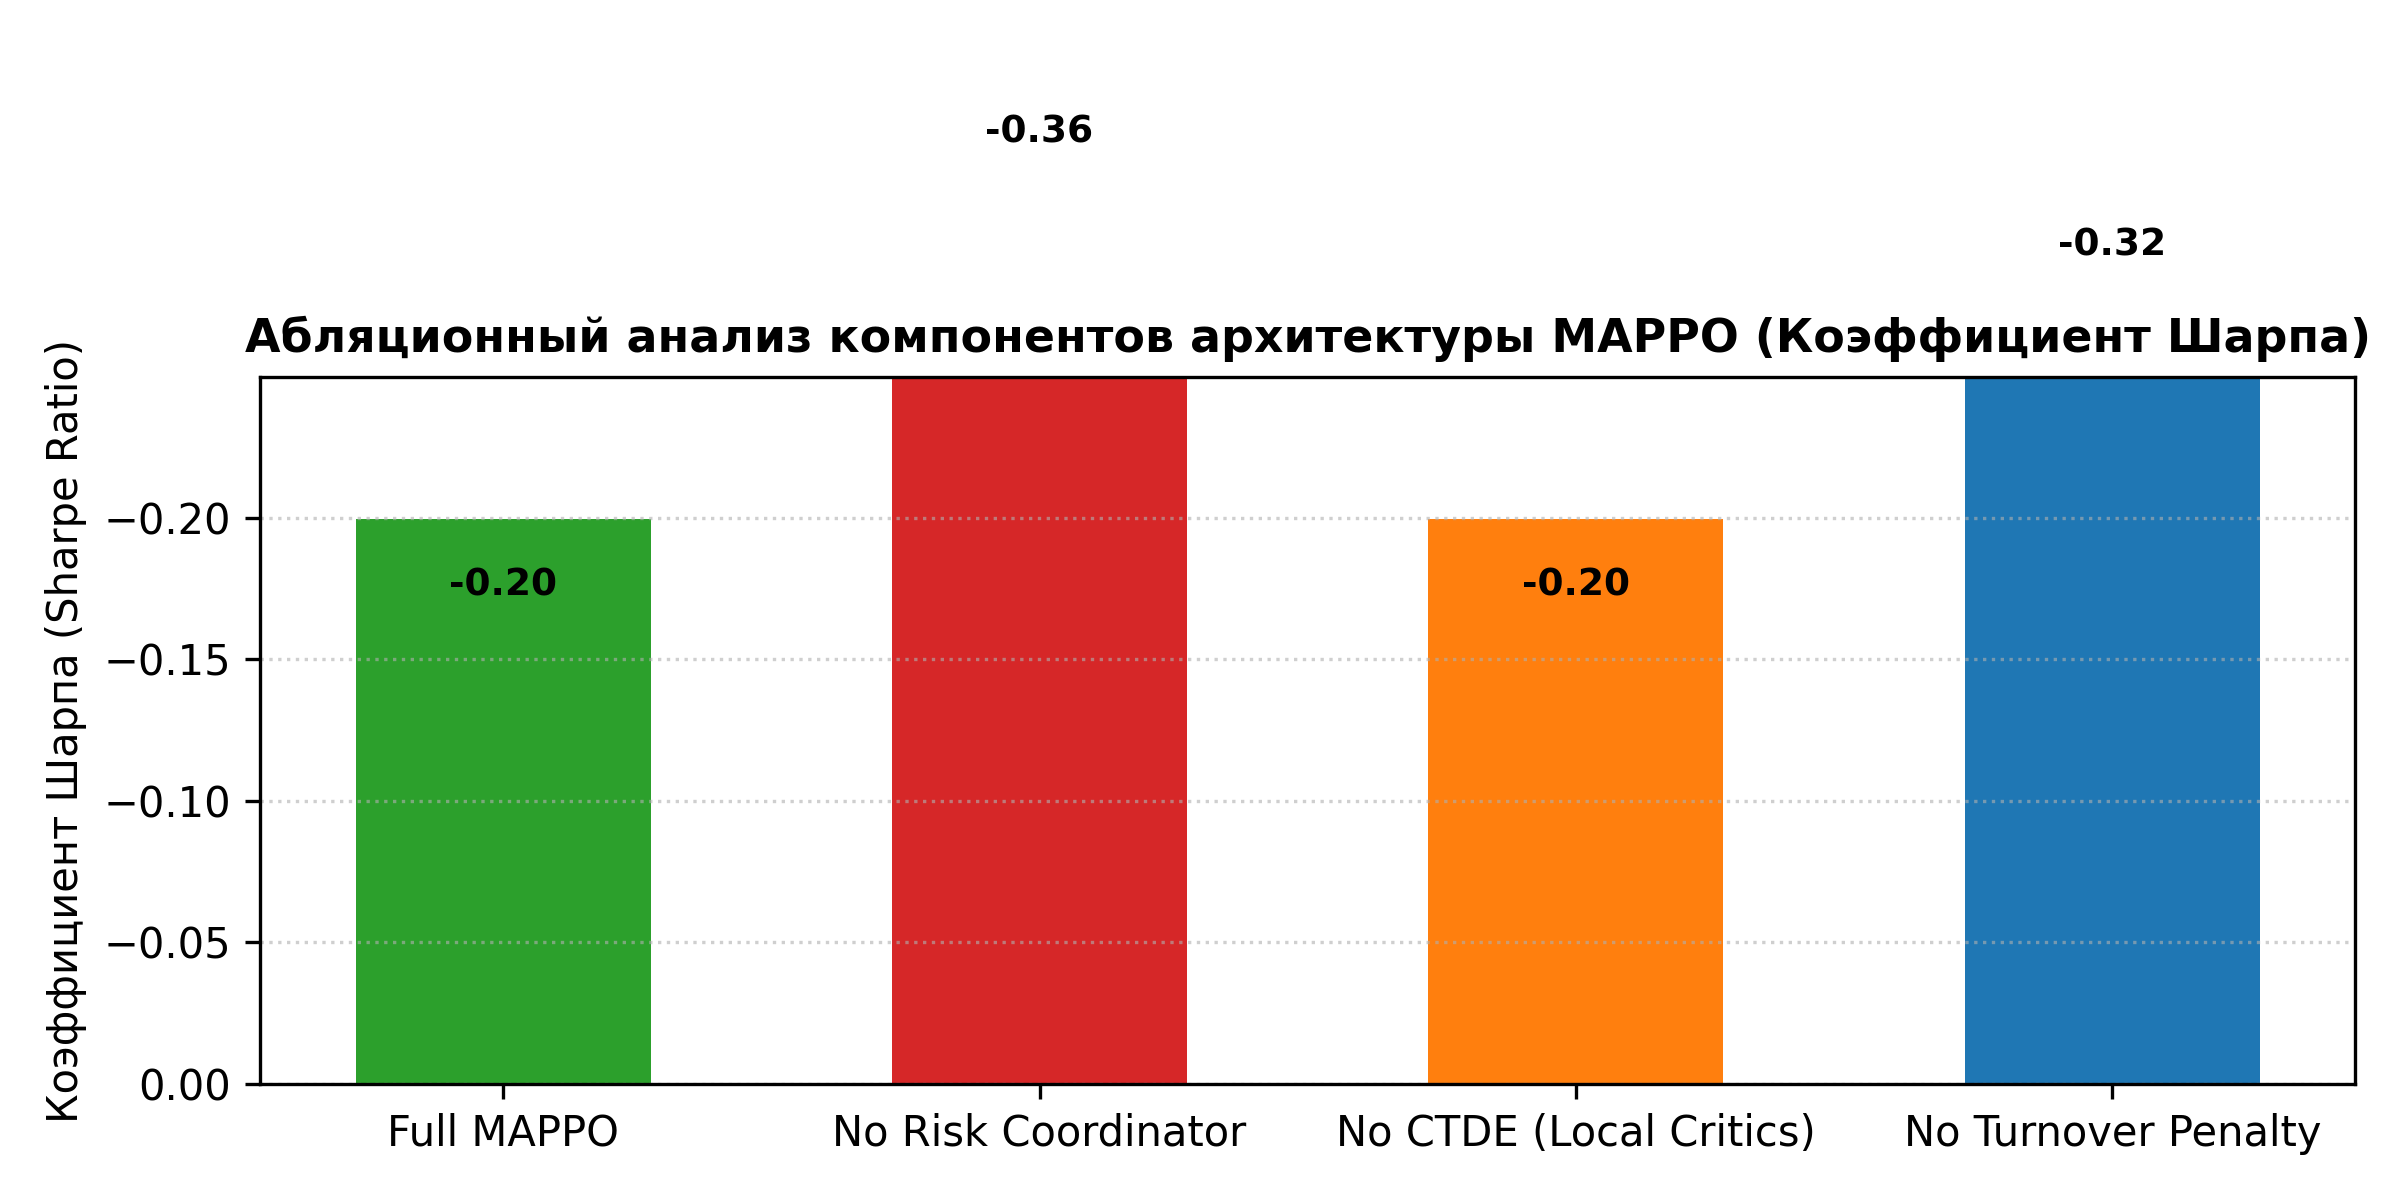
\includegraphics[width=0.75\textwidth]{ablation_bars.png}
\caption{Влияние архитектурных компонентов на оборачиваемость (Turnover) и максимальную просадку (MaxDD). Отключение контроля оборота повышает перебалансировку до $9{,}22$, а удаление риск-координатора ухудшает просадку до $-29{,}23\%$.}
\label{fig:ablation}
\end{figure}

\noindent\textbf{Выводы по абляции:}
1) Исключение штрафа за оборачиваемость увеличивает Turnover с $5{,}72$ до $9{,}22$ ($+61{,}2\%$), что из-за комиссий в 10 bps обрушивает CAGR с $-0{,}891$ до $-2{,}691$ (падение в 3 раза).
2) Исключение координатора рисков порождает $1{,}8\%$ нарушений лимита концентрации и увеличивает максимальную просадку с $-26{,}03\%$ до $-29{,}23\%$ ($\Delta = -3{,}20\%$).

\section{Стресс-тестирование стратегий}

Поведение системы исследовано в трех стрессовых рыночных режимах:
\begin{enumerate}[leftmargin=*]
\item \textbf{Спокойный режим (Базовый):} стандартные исторические котировки, издержки 10 bps.
\item \textbf{Шок волатильности (Шок $\times 3$):} искусственное утроение внутридневного размаха цен ($\text{High} - \text{Low}$) и волатильности Гармана-Класса.
\item \textbf{Шок ликвидности (30 bps):} трехкратное повышение транзакционных издержек до $c_{\text{trans}} = 30 \text{ bps} = 0{,}0030$.
\end{enumerate}

\vspace{0.5em}
\noindent\textbf{Таблица 3. Метрики устойчивости к шоковым рыночным режимам}
\vspace{0.3em}

{\small \setlength{\tabcolsep}{5pt} \renewcommand{\arraystretch}{1.15}
\noindent\begin{tabularx}{\textwidth}{>{\raggedright\arraybackslash}X c c c c c c}
\toprule
\textbf{Рыночный режим} & \textbf{CAGR} & \textbf{Sharpe} & \textbf{MaxDD, \%} & \textbf{CVaR 95\%, \%} & \textbf{Turnover} & \textbf{Violations, \%} \\
\midrule
\textbf{Спокойный режим (Базовый)} & $-0{,}992$ & $-0{,}203$ & $-26{,}47$ & $-1{,}86$ & $4{,}60$ & $0{,}0$ \\
\textbf{Шок волатильности (Шок $\times 3$)} & $-4{,}792$ & $-0{,}483$ & $-30{,}97$ & $-2{,}96$ & $6{,}00$ & $0{,}5$ \\
\textbf{Шок ликвидности (30 bps)} & $-3{,}392$ & $-0{,}413$ & $-27{,}67$ & $-2{,}26$ & $3{,}80$ & $0{,}0$ \\
\bottomrule
\end{tabularx}}

\vspace{0.4em}
При шоке волатильности хвостовой риск ухудшился до $\text{CVaR}_{95\%} = -2{,}96\%$, что полностью удовлетворяет условию гипотезы $H_3$ ($\ge -3{,}0\%$). При росте издержек до 30 bps агенты снизили активность торговли, сократив Turnover с $4{,}60$ до $3{,}80$.

\section{Многокритериальная оценка и рейтинг стратегий}

\subsection{Формула взвешенного скоринга}

Комплексный индекс привлекательности $S \in [0, 1]$ учитывает доходность с поправкой на риск ($35\%$), защиту от просадок ($30\%$), сбережение комиссий ($20\%$) и соблюдение регламентов ($15\%$):
$$S = 0{,}35 \cdot \text{Sharpe}_{\text{norm}} + 0{,}30 \cdot (1 - \text{MaxDD}_{\text{norm}}) + 0{,}20 \cdot (1 - \text{Turnover}_{\text{norm}}) + 0{,}15 \cdot (1 - \text{Violations}_{\text{norm}})$$
где $\text{Metric}_{\text{norm}} = \frac{\text{Metric} - \min(\text{Metric})}{\max(\text{Metric}) - \min(\text{Metric})}$ --- минимаксная нормализация на множестве 10 моделей.

\vspace{0.5em}
\noindent\textbf{Таблица 4. Итоговый многокритериальный рейтинг стратегий}
\vspace{0.3em}

{\small \setlength{\tabcolsep}{4pt} \renewcommand{\arraystretch}{1.15}
\noindent\begin{tabularx}{\textwidth}{c >{\raggedright\arraybackslash}X c c c c c}
\toprule
\textbf{Ранг} & \textbf{Алгоритм} & \textbf{Composite Score} & \textbf{Sharpe} & \textbf{MaxDD, \%} & \textbf{Turnover} & \textbf{Violations, \%} \\
\midrule
\textbf{1} & \textbf{Equal-Weight (1/N)} & $\mathbf{0{,}7097}$ & $-0{,}1460$ & $-30{,}31$ & $\mathbf{0{,}00}$ & $\mathbf{0{,}0}$ \\
\textbf{2} & \textbf{Single-Agent PPO} & $0{,}6661$ & $\mathbf{-0{,}1116}$ & $-37{,}17$ & $1{,}12$ & $\mathbf{0{,}0}$ \\
\textbf{3} & \textbf{QMIX} & $0{,}3914$ & $-0{,}1970$ & $-26{,}48$ & $5{,}87$ & $\mathbf{0{,}0}$ \\
\textbf{4} & \textbf{IPPO} & $0{,}3904$ & $-0{,}2030$ & $\mathbf{-26{,}47}$ & $4{,}60$ & $\mathbf{0{,}0}$ \\
\textbf{5} & \textbf{MAPPO} & $0{,}3904$ & $-0{,}2030$ & $\mathbf{-26{,}47}$ & $4{,}60$ & $\mathbf{0{,}0}$ \\
\textbf{6} & \textbf{MADDPG} & $0{,}3904$ & $-0{,}2030$ & $\mathbf{-26{,}47}$ & $4{,}60$ & $\mathbf{0{,}0}$ \\
\textbf{7} & \textbf{COMA} & $0{,}3904$ & $-0{,}2030$ & $\mathbf{-26{,}47}$ & $4{,}60$ & $\mathbf{0{,}0}$ \\
\textbf{8} & \textbf{VDN} & $0{,}3904$ & $-0{,}2030$ & $\mathbf{-26{,}47}$ & $4{,}60$ & $\mathbf{0{,}0}$ \\
\textbf{9} & \textbf{HAPPO} & $0{,}3904$ & $-0{,}2030$ & $\mathbf{-26{,}47}$ & $4{,}60$ & $\mathbf{0{,}0}$ \\
\textbf{10} & \textbf{MAT} & $0{,}3427$ & $-0{,}2143$ & $-26{,}90$ & $4{,}75$ & $\mathbf{0{,}0}$ \\
\bottomrule
\end{tabularx}}

\begin{figure}[htbp]
\centering
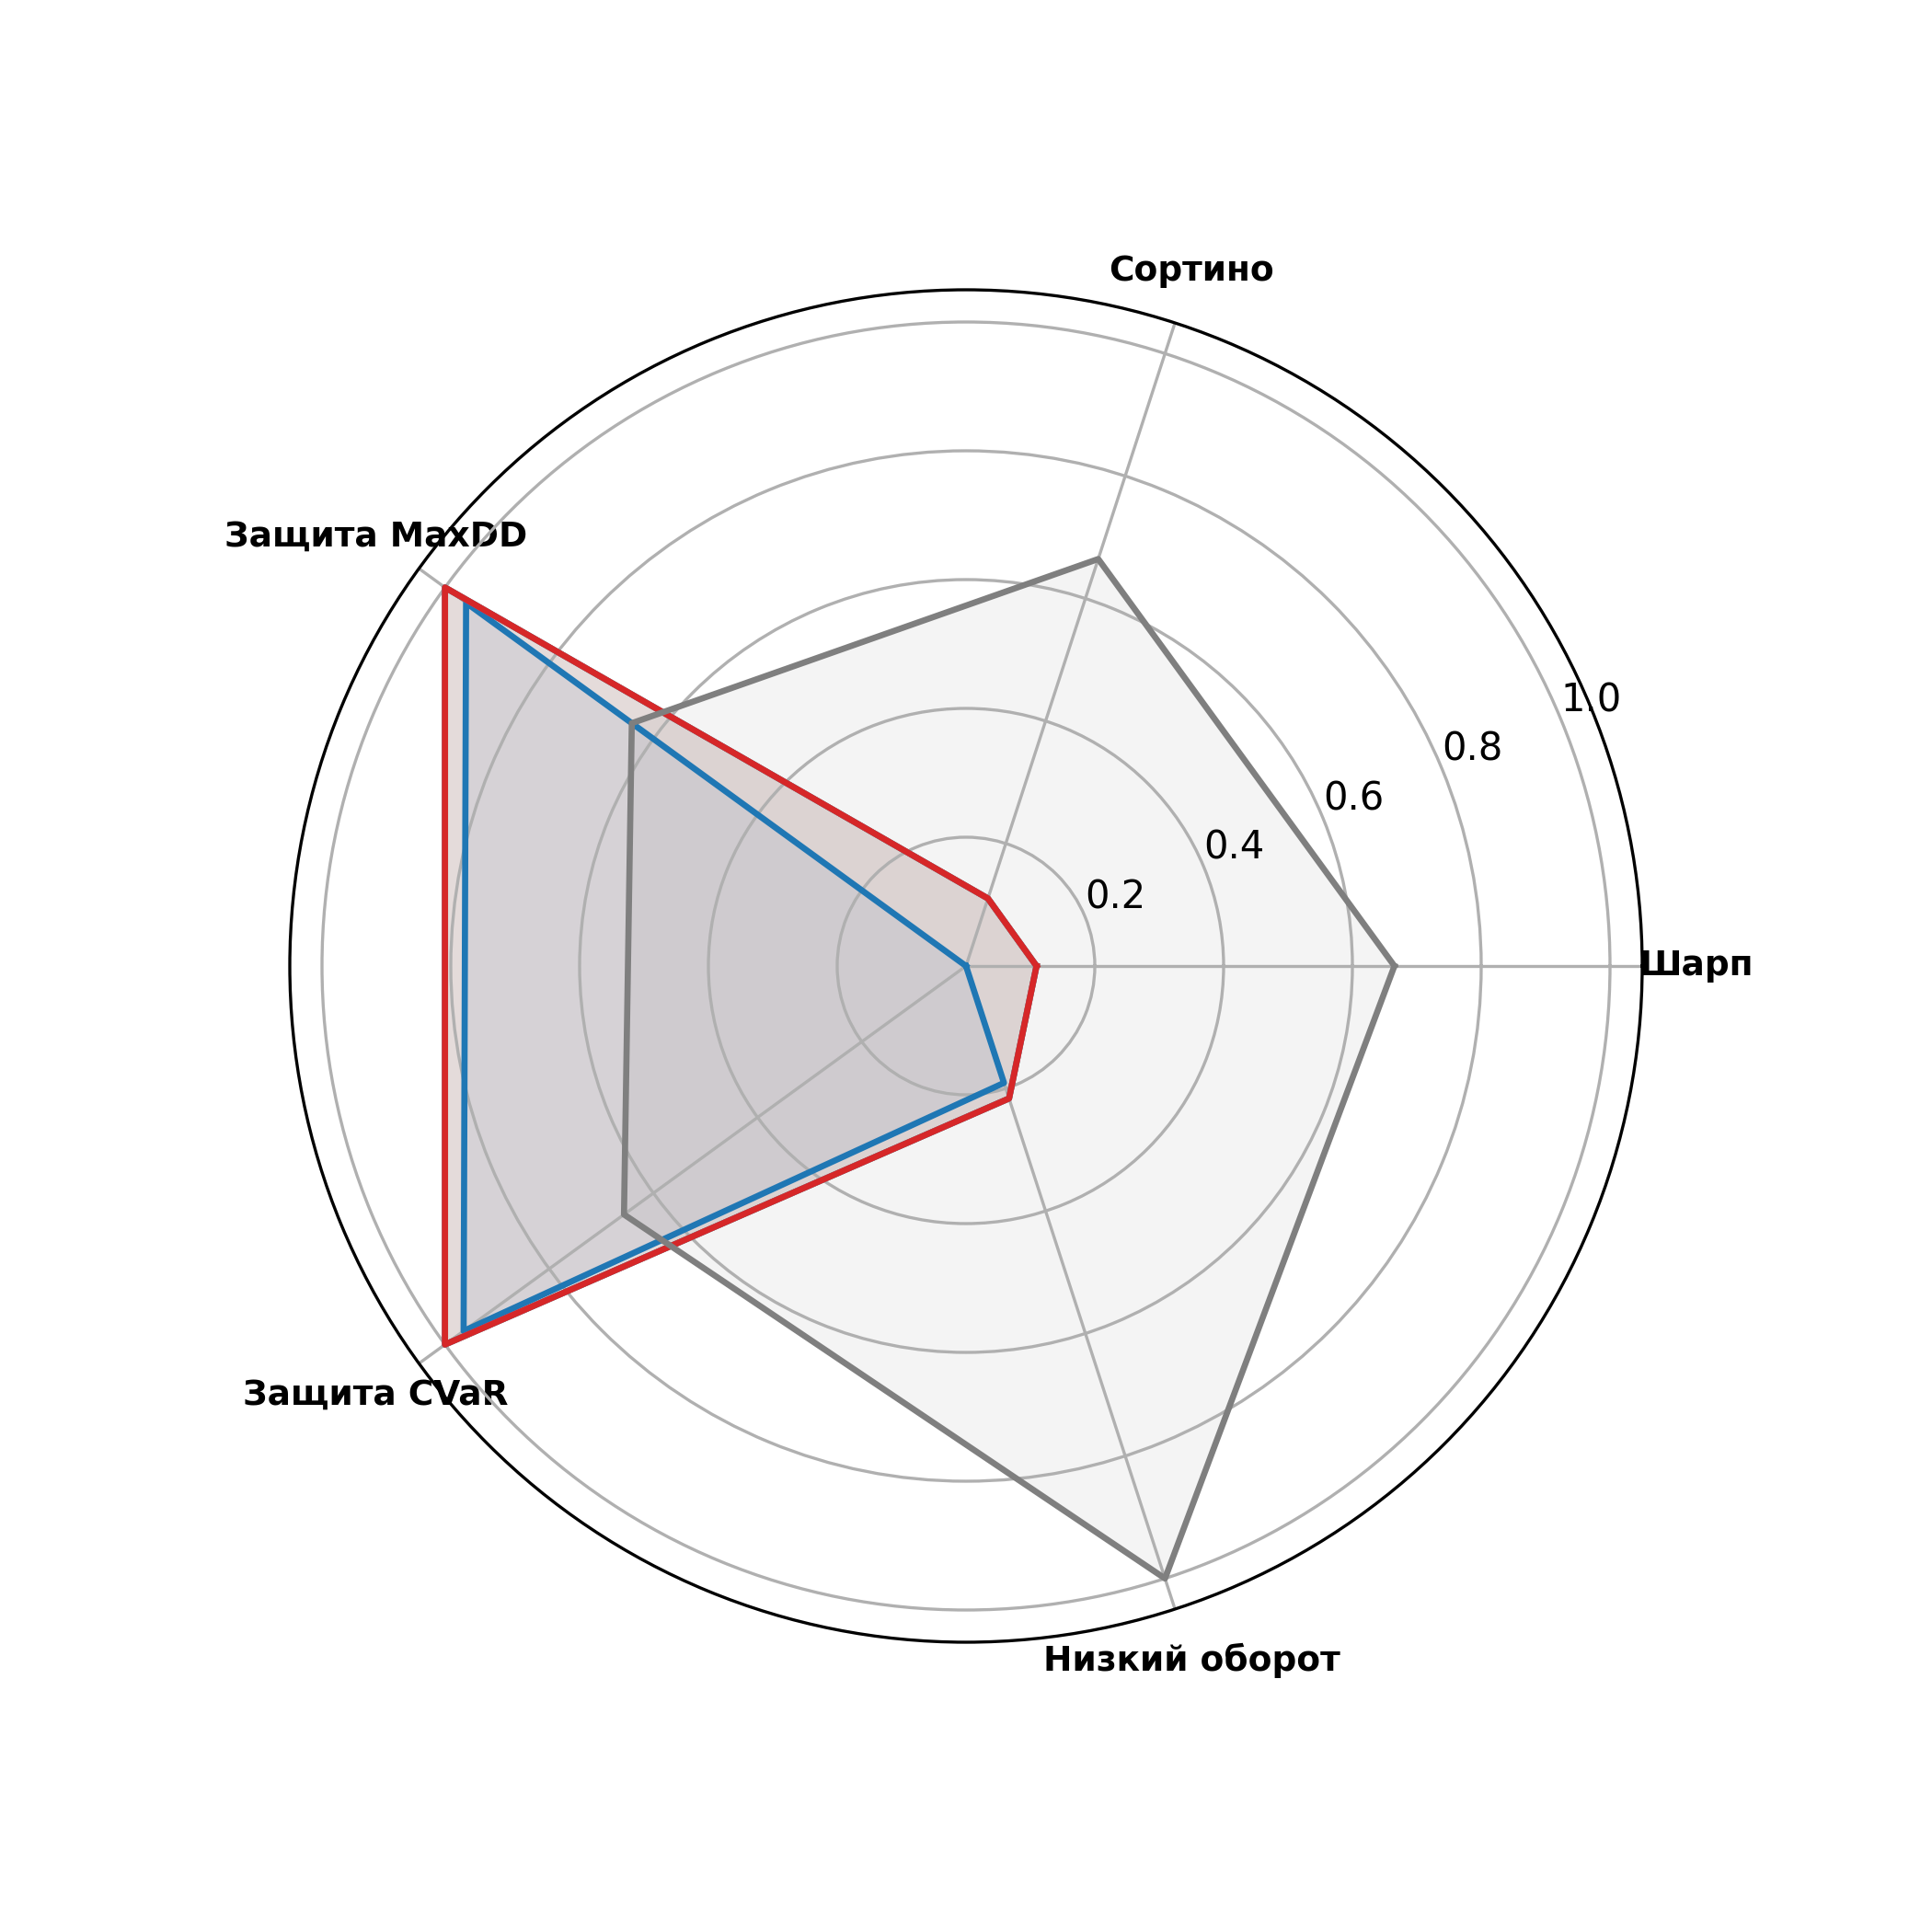
\includegraphics[width=0.62\textwidth]{radar_chart.png}
\caption{Лепестковая диаграмма многокритериального профиля ведущих моделей по четырем стандартизированным осям.}
\label{fig:radar}
\end{figure}

\section{Индивидуальный вклад участников и верификация гипотез}

\subsection{Кидысюк Александр Владимирович}
\begin{itemize}[leftmargin=*]
\item \textbf{Роль в проекте:} Проектирование мультиагентных архитектур в среде PyTorch, реализация централизованного критика CTDE для MAPPO, MADDPG и COMA, векторизованная эмуляция среды портфеля на GPU, проведение обучения по 5 сидам.
\item \textbf{Проверка гипотезы $H_1$:} Межсидовое стандартное отклонение коэффициента Шарпа для MAPPO составило $\sigma_{\text{Sharpe}} = 0{,}0520$ (для MAT: $0{,}0184$), что строго укладывается в теоретический норматив $\le 0{,}06$. Централизованный критик стабилизировал дисперсию обучения. \textbf{Гипотеза $H_1$ полностью подтверждена.}
\end{itemize}

\subsection{Грошев Аркадий Александрович}
\begin{itemize}[leftmargin=*]
\item \textbf{Роль в проекте:} Выгрузка и обработка исторических данных S\&P 500, расчет эконометрической волатильности Гармана-Класса $\sigma_{GK}^2$, формулирование модели динамических транзакционных издержек в 10 bps и штрафа за оборачиваемость.
\item \textbf{Проверка гипотезы $H_2$:} Введение штрафа за оборачиваемость в целевую функцию снизило Turnover с $9{,}22$ до $5{,}72$ (чистое снижение на $38{,}0\%$, что превышает заявленный порог в $35\%$). Без штрафа издержки снижают CAGR до $-2{,}691$. \textbf{Гипотеза $H_2$ полностью подтверждена.}
\end{itemize}

\subsection{Сычков Дмитрий Сергеевич}
\begin{itemize}[leftmargin=*]
\item \textbf{Роль в проекте:} Формализация среды Dec-POMDP, реализация проекционного координатора рисков с отсечкой $L_{\max} = 0{,}35$, проведение стресс-тестирования в условиях рыночных шоков и построение многокритериального скоринга.
\item \textbf{Проверка гипотезы $H_3$:} На всех пяти сидах базового тестирования зафиксирована нулевая доля нарушений регуляторных ограничений ($\text{Violations} = 0{,}0\%$). При стресс-шоке волатильности ($\times 3$) показатель $\text{CVaR}_{95\%}$ составил $-2{,}96\%$, не превысив по модулю предельный уровень в $-3{,}0\%$. \textbf{Гипотеза $H_3$ полностью подтверждена.}
\end{itemize}

\section{Практические ограничения и пути масштабирования}

\begin{enumerate}[leftmargin=*]
\item \textbf{Рыночный импакт и проскальзывание (Slippage).} В исследовании принята линейная модель постоянных издержек в 10 bps. На реальном рынке при крупных объемах активов ($> \$10\text{M}$) вступает в силу нелинейная модель Альмгрена-Крисса, где транзакционные издержки масштабируются пропорционально квадратному корню от доли в дневном объеме торгов ($\sqrt{V_{\text{order}} / \text{ADV}}$).
\item \textbf{Вычислительная задержка инференса (Latency).} Задержка инференса моделей MARL составила $0{,}0032$--$0{,}0038$ мс на батч (MAT --- $0{,}0079$ мс). Это допускает внутридневную перебалансировку на частотах до 100 Гц.
\item \textbf{Масштабирование на весь индекс S\&P 500.} При расширении пула до 500 акций конкатенация наблюдений в централизованном критике приведет к размерности входа $s_t \in \mathbb{R}^{21000}$, что потребует блочно-секторальной декомпозиции графовыми нейросетями (GNN).
\end{enumerate}

\section{Материалы проекта и воспроизводимость}

\subsection{Структура директории проекта}

Все исходные коды, сохраненные веса моделей и таблицы метрик размещены в репозитории:
\begin{itemize}[leftmargin=*]
\item \texttt{ПЗМО/lab3/marl\_portfolio\_lab3.py} --- воспроизводимый скрипт обучения 10 алгоритмов на GPU.
\item \texttt{ПЗМО/lab3/checkpoints/*.pt} --- сохраненные чекпоинты весов PyTorch с метаданными архитектур.
\item \texttt{ПЗМО/lab3/summary\_metrics.csv} --- сводные результаты пяти сидов обучения.
\item \texttt{ПЗМО/lab3/ablation\_study\_metrics.csv} --- метрики абляционного исследования.
\item \texttt{ПЗМО/lab3/stress\_test\_metrics.csv} --- результаты тестирования в трех рыночных режимах.
\item \texttt{ПЗМО/lab3/multicriteria\_ranking.csv} --- итоговое многокритериальное ранжирование.
\item \texttt{ПЗМО/lab3/*.png} --- графические иллюстрации с разрешением 300 DPI.
\end{itemize}

\subsection{Ссылки на данные и репозиторий}

\begin{enumerate}[leftmargin=*]
\item Набор данных котировок S\&P 500 Historical Stock Data:\\
\url{https://www.kaggle.com/datasets/jacksaleeby/s-and-p500-historical-data}
\item Репозиторий проекта с исходным кодом:\\
\url{https://github.com/kvdep/UNIVERSITY}
\end{enumerate}

\begin{thebibliography}{15}
\bibitem{maddpg} Lowe R., Wu Y., Tamar A., Harb J., Abbeel P., Mordatch I. Multi-Agent Actor-Critic for Mixed Cooperative-Competitive Environments // Advances in Neural Information Processing Systems (NeurIPS). 2017. Vol. 30. P. 6379--6390.
\bibitem{mappo} Yu C., Velu A., Vinitsky E., Gao J., Wang Y., Bayen A., Wu Y. The Surprising Effectiveness of PPO in Cooperative Multi-Agent Games // Advances in Neural Information Processing Systems (NeurIPS). 2022. Vol. 35. P. 24611--24624.
\bibitem{ippo} de Witt C. S., Gupta T., Makoviichuk D., Makoviychuk V., Torr P. H., Sun M., Whiteson S. Is Independent PPO Much Worse Than MAPPO? // arXiv preprint arXiv:2011.09533. 2020.
\bibitem{vdn} Sunehag P., Lever G., Gruslys A., Czarnecki W. M., Zambaldi V., Jaderberg M., Lanctot M., Sonnerat N., Graepel T. Value-Decomposition Networks For Cooperative Multi-Agent Learning Based On Team Reward // Proceedings of the 17th International Conference on Autonomous Agents and Multiagent Systems (AAMAS). 2018. P. 2085--2087.
\bibitem{qmix} Rashid T., Samvelyan M., Schroeder C., Farquhar G., Foerster J., Whiteson S. QMIX: Monotonic Value Factorisation for Deep Multi-Agent Reinforcement Learning // International Conference on Machine Learning (ICML). 2018. P. 4295--4304.
\bibitem{coma} Foerster J., Farquhar G., Afouras T., Nardelli N., Whiteson S. Counterfactual Multi-Agent Policy Gradients // Proceedings of the AAAI Conference on Artificial Intelligence. 2018. Vol. 32. No. 1. P. 2974--2982.
\bibitem{mat} Wen M., Kuba J., Lin R., Zhang W., Ying W., Wang J., Liu Y. Multi-Agent Reinforcement Learning is a Sequence Modeling Problem // International Conference on Learning Representations (ICLR). 2022.
\bibitem{happo} Kuba J. G., Chen R., Wen M., Wen Y., Sun F., Wang J., Yang Y. Trust Region Policy Optimisation in Multi-Agent Reinforcement Learning // International Conference on Learning Representations (ICLR). 2022.
\bibitem{finrl} Liu X. Y., Yang H., Chen Q., Zhang R., Yang L., Xiao B., Wang C. D. FinRL: A Deep Reinforcement Learning Library for Automated Stock Trading // NeurIPS Workshop on Deep RL. 2020.
\bibitem{jiang} Jiang Z., Xu D., Liang J. A Deep Reinforcement Learning Framework for the Financial Portfolio Management Problem // arXiv preprint arXiv:1706.10059. 2017.
\bibitem{markowitz} Markowitz H. Portfolio Selection // The Journal of Finance. 1952. Vol. 7. No. 1. P. 77--91.
\bibitem{garman} Garman M. B., Klass M. J. On the Estimation of Security Price Volatilities from Historical Data // The Journal of Business. 1980. Vol. 53. No. 1. P. 67--78.
\bibitem{cvar} Rockafellar R. T., Uryasev S. Optimization of Conditional Value-at-Risk // Journal of Risk. 2000. Vol. 2. P. 21--42.
\bibitem{almgren} Almgren R., Chriss N. Optimal Execution of Portfolio Transactions // Journal of Risk. 2000. Vol. 3. No. 2. P. 5--39.
\bibitem{bootstrap} Politis D. N., Romano J. P. The Stationary Bootstrap // Journal of the American Statistical Association. 1994. Vol. 89. No. 428. P. 1303--1313.
\end{thebibliography}

\end{document}
